\documentclass[11pt,letterpaper,oneside]{book}
\usepackage[utf8]{inputenc}
\usepackage[T1]{fontenc}
\usepackage{lmodern,microtype}
\usepackage[margin=0.90in,headheight=15pt]{geometry}
\usepackage{booktabs,longtable,array,tabularx,multirow}
\usepackage{graphicx,enumitem,xcolor,amsmath,amssymb}
\usepackage[most]{tcolorbox}
\usepackage{tikz}
\usetikzlibrary{arrows.meta,positioning,shapes.geometric,fit,backgrounds}
\usepackage{listings}
\usepackage{fancyhdr,titlesec,xurl,hyperref,bookmark}
\usepackage{lastpage}
\definecolor{navy}{HTML}{17324D}
\definecolor{azure}{HTML}{18638B}
\definecolor{muted}{HTML}{526577}
\definecolor{papergray}{HTML}{F1F5F8}
\definecolor{codegray}{HTML}{F7F8FA}
\definecolor{warn}{HTML}{A45A1A}
\hypersetup{colorlinks=true,linkcolor=navy,urlcolor=azure,citecolor=azure,pdftitle={CodeQL Source Code Security Assessment},pdfauthor={Application Security Engineering Technical Guide}}
\titleformat{\chapter}[display]{\normalfont\sffamily\huge\bfseries\color{navy}}{\large\color{azure}CHAPTER \thechapter}{0.5em}{}
\titleformat{\section}{\normalfont\sffamily\Large\bfseries\color{navy}}{\thesection}{0.8em}{}
\titleformat{\subsection}{\normalfont\sffamily\large\bfseries\color{azure}}{\thesubsection}{0.8em}{}
\setlist[itemize]{noitemsep,topsep=3pt,leftmargin=1.5em}
\setlist[enumerate]{topsep=3pt,itemsep=2pt,leftmargin=1.7em}
\pagestyle{fancy}\fancyhf{}\lhead{\small\sffamily CodeQL Security Assessment}\rhead{\small\sffamily Engineering Guide}\cfoot{\small\thepage\ / \pageref{LastPage}}
\renewcommand{\headrulewidth}{0.35pt}
\newtcolorbox{infobox}[1]{enhanced,colback=papergray,colframe=azure!65,boxrule=0.7pt,title={#1},fonttitle=\bfseries\sffamily,coltitle=white,colbacktitle=navy,breakable,arc=2pt,top=5pt,bottom=5pt}
\lstdefinestyle{tech}{basicstyle=\ttfamily\footnotesize,keywordstyle=\color{azure}\bfseries,commentstyle=\color{muted}\itshape,stringstyle=\color{warn},backgroundcolor=\color{codegray},frame=single,rulecolor=\color{navy!15},breaklines=true,breakatwhitespace=false,showstringspaces=false,columns=fullflexible,keepspaces=true,tabsize=2,captionpos=b,xleftmargin=4pt,xrightmargin=4pt,aboveskip=9pt,belowskip=9pt}
\lstset{style=tech}
\newcommand{\srcB}{\textsf{[Bishop, textbook]}}
\newcommand{\srcD}{\textsf{[Dowd--McDonald--Schuh, textbook]}}
\newcommand{\srcM}{\textsf{[Modern CodeQL documentation]}}
\newcommand{\srcR}{\textsf{[Engineering recommendation]}}
\newcommand{\limt}{\textsf{[Assessment limitation]}}
\begin{document}
\frontmatter
\begin{titlepage}
\thispagestyle{empty}
\vspace*{0.7in}
{\sffamily\Large\color{azure} SOFTWARE SECURITY ENGINEERING / TECHNICAL REFERENCE}\par\vspace{0.55in}
{\sffamily\fontsize{32}{38}\selectfont\bfseries\color{navy} CODEQL SOURCE CODE\\SECURITY ASSESSMENT}\par
\vspace{0.32in}
{\sffamily\Large Security Foundations, Static Analysis, Vulnerability Validation, and Enterprise Implementation}\par
\vspace{0.85in}\noindent\color{azure}\rule{\linewidth}{1.5pt}\par\vspace{0.4in}
\begin{tabular}{ll}
\textbf{Edition} & 1.0 --- 16 October 2026 \\
\textbf{Audience} & Application security engineers, reviewers, CodeQL engineers \\
\textbf{Source basis} & Bishop (2019); Dowd, McDonald \& Schuh (2007) \\
\textbf{Implementation} & CodeQL / GitHub code scanning; official docs reviewed 2026-10-16 \\
\textbf{Validation} & LaTeX compiled; CodeQL query execution not available locally
\end{tabular}
\vfill
{\small\color{muted}Original technical synthesis for authorized, defensive code assessment. This document does not certify any repository as secure. Product behavior is version- and configuration-dependent; validate against the currently deployed toolchain.}\par
\end{titlepage}
\chapter*{Document control}\addcontentsline{toc}{chapter}{Document control}
\begin{tabularx}{\linewidth}{l l X}
\toprule Version & Date & Change summary \\\midrule
1.0 & 2026-10-16 & Initial textbook-grounded assessment method, CodeQL implementation reference, catalog, workflows, reporting, laboratories.\\\bottomrule
\end{tabularx}
\vspace{10pt}
\begin{infobox}{Scope and evidence status}
This is a methodology and reference handbook, \emph{not} a completed security assessment of a live repository. All hypothetical findings are examples; no organizational inventory, CodeQL execution output, tool versions, or exploit demonstrations were supplied. CodeQL CLI is not installed in the authoring environment: example QL queries are documentation-derived and \textbf{not locally compiled or exercised}. Where the guide describes organizational policy it is a proposed standard, not a GitHub mandate.
\end{infobox}
\tableofcontents
\listoffigures
\listoftables
\lstlistoflistings
\mainmatter
\chapter{Foundations of Software Security Assessment}

\section{Security as an explicit policy claim}

\srcB\ Bishop, Chapter 1, treats confidentiality, integrity, and availability as related but distinct security goals. A code assessment starts by describing \emph{assets}, \emph{authorized behavior}, \emph{adversary capabilities}, and \emph{assumptions}. A vulnerability is therefore not just a suspicious syntax tree: it is a feasible deviation from an intended security requirement or an unsafe behavior that contributes to such deviation.

The analyst should write a falsifiable statement such as: ``A tenant may read only documents belonging to that tenant, regardless of route parameters.'' The policy may be enforced by middleware, database predicates, or application code. These are \emph{mechanisms}; their existence does not establish that the requirement is enforced on every reachable path. \srcR\ Record an asset--operation--principal--condition tuple for each critical boundary.

\section{Threat model and assessment unit}

\begin{itemize}
\item \textbf{Assets:} credentials, personal data, financial records, execution privileges, service availability, and integrity of business transactions.
\item \textbf{Entry points:} HTTP routes, queue messages, CLI arguments, environment variables, file uploads, scheduled tasks, RPC endpoints, and internal integration events.
\item \textbf{Trust boundaries:} user to service, service to data store, tenant to tenant, privileged to unprivileged component, and CI job to deployment credential.
\item \textbf{Adversary:} anonymous remote caller, authenticated user, compromised dependency, malicious contributor, or privileged insider; define their actual control.
\item \textbf{Assumptions:} identity from middleware, signature verification, object ownership, deployment flags, authorization middleware order, and network isolation.
\end{itemize}

\section{Assurance and uncertainty}

\srcB\ Bishop Chapters 19--20 separate requirements, design, implementation, and operational evidence. In a SAST assessment, evidence is layered: the extraction must be usable, the relevant query must run, the flow model must represent the application, and the analyst must test the security conclusion. A clean CodeQL run increases confidence for \emph{modeled} weaknesses but cannot prove overall safety.

\begin{infobox}{Finding confidence is not exploitability}
A CodeQL alert is a \emph{candidate concern}; a path explanation is evidence of a modeled path; a validated vulnerability requires security-context analysis; a demonstrated exploit requires reproducible behavior in an authorized test environment. Never collapse these categories into one status.
\end{infobox}

\section{Assessment claim hierarchy}

\small
\setlength{\tabcolsep}{2pt}
\renewcommand{\arraystretch}{1.18}
\begin{longtable}{>{\raggedright\arraybackslash}p{0.27\linewidth}>{\raggedright\arraybackslash}p{0.68\linewidth}}
\toprule
\textbf{Claim} & \textbf{Minimum defensible evidence}\\
\midrule
\endfirsthead
\toprule
\textbf{Claim} & \textbf{Minimum defensible evidence}\\
\midrule
\endhead
Configured & Workflow/configuration exists; scope and triggers reviewed\\
Executed & Successful run, commit SHA, language, tool and suite captured\\
Coverage characterized & Scope, omitted files, extracted language units, limitations and queries documented\\
Finding validated & Source, propagation, control, sink, privileges and impact examined\\
Remediation verified & Fix review, tests, correct scan context, clean expected result, no equivalent unsafe path\\
Assurance argument & Multiple evidence types plus explicit residual uncertainty\\
\bottomrule
\end{longtable}
\normalsize

\chapter{Secure Design Principles and Code Assessment}

\section{Translating principles into review hypotheses}

\srcB\ The eight principles in Bishop, Section 14.2, concern the \emph{security design of a system}, not just individual instructions. The table below distinguishes CodeQL-discoverable symptoms from policies that require architectural or operational validation.

\small
\setlength{\tabcolsep}{2pt}
\renewcommand{\arraystretch}{1.18}
\begin{longtable}{>{\raggedright\arraybackslash}p{0.17\linewidth}>{\raggedright\arraybackslash}p{0.27\linewidth}>{\raggedright\arraybackslash}p{0.27\linewidth}>{\raggedright\arraybackslash}p{0.24\linewidth}}
\toprule
\textbf{Principle} & \textbf{Failure hypothesis} & \textbf{CodeQL candidate investigation} & \textbf{Manual evidence}\\
\midrule
\endfirsthead
\toprule
\textbf{Principle} & \textbf{Failure hypothesis} & \textbf{CodeQL candidate investigation} & \textbf{Manual evidence}\\
\midrule
\endhead
\textbf{Least privilege} & Background job has administrative credentials & Search privileged APIs, roles and grant operations & Compare effective runtime authority with task requirements\\
\textbf{Fail-safe defaults} & Catch block returns allow=true after policy-service failure & Search unsafe fallback expressions and exception handlers & Verify failure semantics with injected dependency failures\\
\textbf{Economy of mechanism} & Two competing access-control implementations & Find duplicated sensitive operations and bypasses & Trace all authorization paths and consolidate mechanisms\\
\textbf{Complete mediation} & Endpoint accesses records without object ownership check & Locate sensitive sinks and conditional checks & Test each object access with cross-tenant identities\\
\textbf{Open design} & Security assumes URL or client code remains secret & Inventory secrets, hardcoded checks and obscurity-dependent branches & Review threat model and key lifecycle\\
\textbf{Separation of privilege} & High-impact action authorized by one unchecked role claim & Identify approval-related calls and bypass paths & Confirm independent conditions and enforcement\\
\textbf{Least common mechanism} & Shared cache leaks tenant-scoped objects & Search shared caches and keys & Test multi-tenant isolation and cross-request state\\
\textbf{Least astonishment} & Sensitive API unexpectedly logs access tokens & Search logging/serialization of sensitive data & Review user expectations and data retention\\
\bottomrule
\end{longtable}
\normalsize

\section{Working example: complete mediation}

Consider an internal API that receives an authenticated principal but retrieves a customer record solely by an attacker-selected identifier. The defect is \emph{missing record-level authorization}, even when the SQL statement is parameterized. Standard injection queries are not a substitute for this policy review.

\begin{lstlisting}[caption={Python: unscoped and tenant-scoped retrieval},language=Python]
def get_invoice(db, invoice_id):
    return db.execute(
        "SELECT * FROM invoices WHERE id = ?",
        (invoice_id,),
    ).fetchone()

def get_invoice_scoped(db, invoice_id, tenant_id):
    return db.execute(
        "SELECT * FROM invoices WHERE id = ? AND tenant_id = ?",
        (invoice_id, tenant_id),
    ).fetchone()
\end{lstlisting}

The corrected example assumes \texttt{tenant\_id} is derived from authenticated server-side context, not an untrusted client claim. \srcR\ Verify horizontal authorization with two tenant fixtures, deny-by-default behavior, and logging that does not expose the invoice. \limt\ A generalized query cannot reliably infer all business-specific ownership semantics.

\section{Validation examples for other design principles}

\begin{itemize}
\item \textbf{Fail-safe defaults:} force policy-store timeout; require access denied, state rollback, and a traceable failure event.
\item \textbf{Separation of privilege:} use test identities independently lacking each required approval; neither bypass should authorize the transaction.
\item \textbf{Least privilege:} inspect deployment IAM and runtime role credentials, not only the symbolic permissions in source.
\item \textbf{Least common mechanism:} interleave two tenant requests with identical cache keys; check that neither reads the other tenant\textquotesingle s data.
\end{itemize}

\chapter{Vulnerability Taxonomy and Assessment Boundaries}

\section{Three original categories and a modern extension}

\srcD\ Dowd, McDonald, and Schuh, Chapter 1, distinguish \emph{design}, \emph{implementation}, and \emph{operational} vulnerabilities. This guide adds configuration as an operationally useful reporting dimension, not as a replacement for their categories. A flaw may span categories: for example, a hardcoded shared administrator secret may originate in code and become exploitable through deployment configuration.

\small
\setlength{\tabcolsep}{2pt}
\renewcommand{\arraystretch}{1.18}
\begin{longtable}{>{\raggedright\arraybackslash}p{0.18\linewidth}>{\raggedright\arraybackslash}p{0.44\linewidth}>{\raggedright\arraybackslash}p{0.33\linewidth}}
\toprule
\textbf{Type} & \textbf{Example} & \textbf{Primary validation method}\\
\midrule
\endfirsthead
\toprule
\textbf{Type} & \textbf{Example} & \textbf{Primary validation method}\\
\midrule
\endhead
Design & Cross-tenant lookup without ownership model & Architectural analysis and security-invariant tests\\
Implementation & User value concatenated into SQL query & Taint path, call semantics, dynamic test\\
Operational & Missing ingress authentication due to deployment choice & Deployment evidence and authorized environment test\\
Configuration & Excessive workflow token permissions & Workflow inspection and effective permission check\\
\bottomrule
\end{longtable}
\normalsize

\section{CWE relationship and root cause}

MITRE CWE identifies software weakness classes; CVE identifies publicly disclosed vulnerabilities in concrete products when assigned. A single vulnerability may involve multiple CWEs, and a CWE does not prove exploitability. Use the most specific defensible CWE; document uncertainty. Do not infer a CVE from CodeQL output alone. CodeQL rule metadata and CWE tags are useful candidate classifications, but a human reviewer must verify the root cause.

\section{False positives and false negatives}

False positives arise when a model omits sanitization, context, or path constraints. False negatives arise when sources/sinks are unmodeled, generated code or languages are absent from extraction, library summaries are incomplete, or design failures do not match a computable pattern. \srcD\ Dowd et al., Chapter 4, explicitly warn that candidate-point approaches bias review toward the chosen patterns. \srcR\ Include a dedicated negative-space pass: Which high-value security invariants had no direct query coverage?

\chapter{CodeQL Architecture and Execution Model}

\section{Database, query, results, and evidence}

\srcM\ CodeQL extracts language-aware program representations into a database, runs QL queries or suites, and produces query results or SARIF for code-scanning ingestion. This is static reasoning over the code as modeled at extraction time, not runtime execution. Language extractors and libraries differ; no universal AST, CFG, or framework model is guaranteed for all supported languages.

\begin{figure}[htbp]\centering
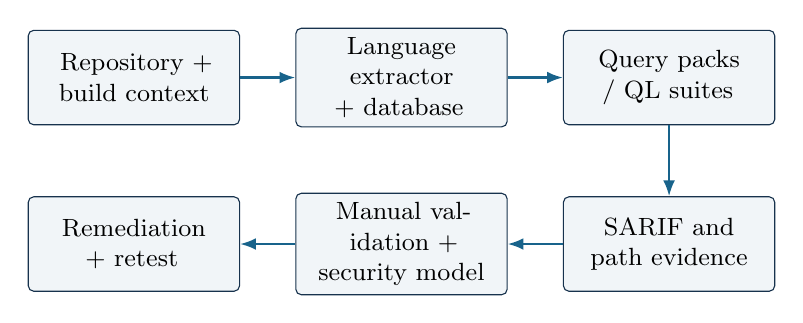
\begin{tikzpicture}[node distance=9mm and 7mm, every node/.style={font=\small}, nodebox/.style={draw=navy,rounded corners=2pt,fill=papergray,text width=2.45cm,minimum height=12mm,align=center}, arr/.style={-{Latex[length=2mm]},thick,draw=azure}]
\node[nodebox](repo){Repository + build context};
\node[nodebox,right=of repo](extract){Language extractor + database};
\node[nodebox,right=of extract](query){Query packs / QL suites};
\node[nodebox,below=of query](sarif){SARIF and path evidence};
\node[nodebox,left=of sarif](review){Manual validation + security model};
\node[nodebox,left=of review](action){Remediation + retest};
\draw[arr](repo)--(extract);\draw[arr](extract)--(query);\draw[arr](query)--(sarif);\draw[arr](sarif)--(review);\draw[arr](review)--(action);
\end{tikzpicture}
\caption{CodeQL extraction, query execution, and human assessment pipeline}\label{fig:pipeline}\end{figure}

\section{Representations and their limitations}

\begin{itemize}
\item \textbf{Syntax / AST:} parse-time nodes support patterns such as calls and binary expressions.
\item \textbf{Control flow:} reachable branches, exception paths, and nodes; language-specific approximations and CFG splitting apply.
\item \textbf{Data flow:} value propagation using data-flow nodes; local analysis is cheaper and typically more precise.
\item \textbf{Taint tracking:} influence propagation across operations that do not preserve exact values, such as string concatenation.
\item \textbf{Interprocedural analysis:} may follow calls and library models within supported limits; reflection, native boundaries, and unknown frameworks require supplemental reasoning.
\item \textbf{Path queries:} provide explanatory steps across modeled flows; presence of a path is not automatically a real exploit.
\end{itemize}

\section{Supported language inventory}

\srcM\ Official built-in query tables enumerate GitHub Actions, C/C++, C\#, Go, Java/Kotlin, JavaScript/TypeScript, Python, Ruby, Rust, and Swift. GitHub Actions analysis is workflow-specific and not a generic executable-language extractor. Verify supported framework and build requirements for each repository before asserting coverage. See the bibliography for current documentation URLs.

\section{Extraction and compilation}

\srcM\ GitHub supports \texttt{none}, \texttt{autobuild}, and \texttt{manual} modes where applicable. No-build mode is available for supported interpreted languages and selected compiled languages (currently C/C++, C\#, Java and Rust). Language- and project-specific dependencies can affect extraction quality. Kotlin requires a build-capable mode. Preserve extraction logs and resolved source inventory when performing compliance audits.

\section{Result format and provenance}

Every assessment artifact should preserve the repository URL, commit SHA, branch/ref, execution time, CodeQL version, query pack/suite and custom pack lockfile, tool configuration, event type, result category, SARIF file hash, and run URL. Avoid relying exclusively on a mutable dashboard snapshot.

\chapter{Developing CodeQL Queries}

\section{QL constructs and query precision}

QL provides declarative classes, predicates, logical constraints, quantification, recursion, and relations over an extracted program. Use a simple syntax/usage query to inventory candidates; use data-flow/taint queries to constrain their causal relationship to untrusted sources. Modern Python analysis uses the modular \texttt{DataFlow::ConfigSig} API rather than removed legacy configuration classes. \srcM\ Examples below are derived from the official language guide and path-query documentation, but were \textbf{not compiled locally}.

\subsection{Query A: filesystem call inventory}

\begin{lstlisting}[caption={CodeQL/Python: candidate-point query from official API idioms}]
/**
 * @name File-opening operations for manual audit
 * @description Inventories calls to os.open for path review.
 * @kind problem
 * @problem.severity recommendation
 * @id py/example/file-open-inventory
 */
import python
import semmle.python.dataflow.new.DataFlow
import semmle.python.ApiGraphs

from DataFlow::CallCfgNode call
where
  call = API::moduleImport("os").getMember("open").getACall()
select call, "Inspect this file-opening operation and its caller context."
\end{lstlisting}

This query inventories a sensitive operation, \emph{not} path traversal vulnerabilities. A legitimate file-open call will also appear. The reviewer must determine attacker influence and path restriction. Official syntax used here is documented in \url{https://codeql.github.com/docs/codeql-language-guides/analyzing-data-flow-in-python/}.

\subsection{Query B: local taint from function parameters to file paths}

\begin{lstlisting}[caption={CodeQL/Python: local candidate flow}]
/**
 * @name Function parameter influences os.open path
 * @description Identifies local taint candidates for manual review.
 * @kind problem
 * @problem.severity warning
 * @id py/example/parameter-to-file-path
 */
import python
import semmle.python.dataflow.new.TaintTracking
import semmle.python.ApiGraphs

from DataFlow::CallCfgNode call, DataFlow::ParameterNode p
where
  call = API::moduleImport("os").getMember("open").getACall() and
  TaintTracking::localTaint(p, call.getArg(0))
select call, "A function parameter influences this path argument."
\end{lstlisting}

The parameter may be internal and trusted. A local taint path is therefore an investigation lead. Review all callers, trust-boundary origins and canonicalization/allowlist logic. When the question concerns network-sourced input across call boundaries, use a global, scoped query.

\subsection{Query C: global path query configuration}

\begin{lstlisting}[caption={CodeQL/Python: documentation-derived global path query}]
/**
 * @name Remote input can influence a filesystem path
 * @description Tracks modeled network sources to filesystem paths.
 * @kind path-problem
 * @problem.severity warning
 * @id py/example/remote-to-file
 */
import python
import semmle.python.dataflow.new.DataFlow
import semmle.python.dataflow.new.TaintTracking
import semmle.python.dataflow.new.RemoteFlowSources
import semmle.python.Concepts

module Config implements DataFlow::ConfigSig {
  predicate isSource(DataFlow::Node source) {
    source instanceof RemoteFlowSource
  }
  predicate isSink(DataFlow::Node sink) {
    sink = any(FileSystemAccess fa).getAPathArgument()
  }
}
module Flow = TaintTracking::Global<Config>;
import Flow::PathGraph

from Flow::PathNode source, Flow::PathNode sink
where Flow::flowPath(source, sink)
select sink.getNode(), source, sink,
  "Remote data can influence this path; review authorization and containment."
\end{lstlisting}

This query is deliberately broader than a vulnerability detector. It does not require a path traversal operation, unsafe file mode, or absence of sanitization; it will include legitimate uses. Before enabling it in production, run isolated fixtures, tune sinks, model application-specific barriers, and measure false positives. For precise query metadata and path selection consult the official ``Creating path queries'' guide.

\section{Query engineering quality gates}

\begin{itemize}
\item \textbf{Correctness:} use version-pinned CodeQL libraries; compile queries; ensure the result location and path nodes are valid.
\item \textbf{Positive fixture:} known unsafe path triggers expected query result.
\item \textbf{Negative fixture:} valid secured path does not trigger (or is explicitly identified as intentionally broad).
\item \textbf{Precision:} track true and false positives during pilot rollout; document supported frameworks.
\item \textbf{Performance:} bound broad Cartesian products and use meaningful source/sink constraints.
\item \textbf{Lifecycle:} version queries, test library upgrades, and route coverage gaps back to query authors.
\end{itemize}

\chapter{Analysis Configuration, Completeness, and Coverage}

\section{Decision framework for setup modes}

\srcM\ Default setup offers managed configuration and supported customization; advanced setup is appropriate for custom builds, matrix strategies, custom queries, or organization-specific workflow controls. Both must be validated against repo language composition and build reality.

\small
\setlength{\tabcolsep}{2pt}
\renewcommand{\arraystretch}{1.18}
\begin{longtable}{>{\raggedright\arraybackslash}p{0.24\linewidth}>{\raggedright\arraybackslash}p{0.34\linewidth}>{\raggedright\arraybackslash}p{0.37\linewidth}}
\toprule
\textbf{Criterion} & \textbf{Default setup} & \textbf{Advanced setup}\\
\midrule
\endfirsthead
\toprule
\textbf{Criterion} & \textbf{Default setup} & \textbf{Advanced setup}\\
\midrule
\endhead
Build complexity & Suitable for supported automatic extraction & Explicit multi-stage build, manual build modes\\
Query customisation & Supported managed settings & Fine control with config and packs\\
Operational burden & Lower & Higher; workflow maintenance\\
Evidence & Configuration and managed run records & Versioned YAML, runners and build logs\\
Decision & Baseline where adequate & Use for requirements default cannot meet\\
\bottomrule
\end{longtable}
\normalsize

\section{CLI workflow for reproducible local assessment}

\begin{lstlisting}[caption={Illustrative CLI sequence; confirm suite syntax against installed bundle},language=bash]
# Confirm tool availability first (not installed in authoring environment)
codeql version
# Run inside an authorized example repository
codeql database create ./codeql-db --language=python --source-root=.
# Use the shipped query suite for the installed pack/version
codeql database analyze ./codeql-db \
  codeql/python-queries:codeql-suites/python-security-extended.qls   --format=sarif-latest --output=results.sarif
# Validate the SARIF run metadata, artifact paths, and rule IDs
\end{lstlisting}

\limt\ Suite paths and pack layout are version-sensitive; use \texttt{codeql resolve queries} and package documentation before copying this workflow into a regulated process. Commands are shown for training, not as evidence of a completed run.

\section{Coverage metrics and explicit exclusions}

Count a repository as \emph{analyzed} only if an expected language scan completed for the target ref and within the organization-defined freshness window. Repositories without supported languages, archived repositories, or approved exclusions belong in separate denominators. A scan job that exits successfully but excludes key generated code or target languages may not meet coverage acceptance criteria.

\begin{lstlisting}[caption={Denominator definitions; handle zero denominator as not applicable}]
eligible = supported - archived - approved_exemptions
coverage_rate = successful_fresh_scans / eligible
language_coverage = successfully_analyzed_language_pairs / eligible_pairs
triage_rate = decisioned_alerts / review_due_alerts
verification_rate = verified_fixes / fixes_awaiting_verification
\end{lstlisting}

\chapter{CodeQL-Assisted Application Assessment Methodology}

\section{Hybrid top-down / bottom-up review}

\srcD\ Dowd et al., Chapter 4, propose iterative preassessment, planning, review work and reflection. Their code-comprehension (CC) strategies seek system understanding; candidate-point (CP) strategies begin with suspicious operations; design-generalization (DG) strategies infer architecture and logic vulnerabilities. This guide implements a \emph{hybrid}: a small threat model drives CodeQL selection, then candidate findings and tracing deepen the threat model.

\begin{figure}[htbp]\centering
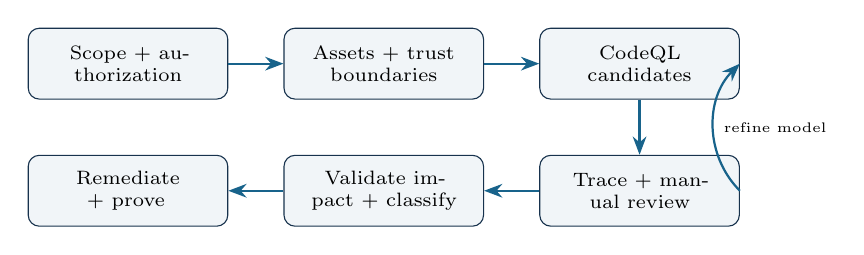
\begin{tikzpicture}[node distance=7mm and 7mm, every node/.style={font=\scriptsize}, st/.style={draw=navy,rounded corners,fill=papergray,minimum height=9mm,text width=2.3cm,align=center}, ar/.style={-{Stealth},draw=azure,thick}]
\node[st](scope){Scope + authorization};\node[st,right=of scope](model){Assets + trust boundaries};\node[st,right=of model](code){CodeQL candidates};\node[st,below=of code](trace){Trace + manual review};\node[st,left=of trace](valid){Validate impact + classify};\node[st,left=of valid](fix){Remediate + prove};
\draw[ar](scope)--(model);\draw[ar](model)--(code);\draw[ar](code)--(trace);\draw[ar](trace)--(valid);\draw[ar](valid)--(fix);\draw[ar] (trace.east) to[bend left=45] node[right]{\tiny refine model} (code.east);
\end{tikzpicture}\caption{Iterative assessment lifecycle combining top-down and candidate-driven review}\label{fig:lifecycle}\end{figure}

\section{Fourteen-step operational playbook}

\small
\setlength{\tabcolsep}{2pt}
\renewcommand{\arraystretch}{1.18}
\begin{longtable}{>{\raggedright\arraybackslash}p{0.28\linewidth}>{\raggedright\arraybackslash}p{0.67\linewidth}}
\toprule
\textbf{Stage} & \textbf{Assessment operation / objective}\\
\midrule
\endfirsthead
\toprule
\textbf{Stage} & \textbf{Assessment operation / objective}\\
\midrule
\endhead
1. Authorize and scope & Identify owner, target refs, permitted tests, confidentiality classification, exclusions.\\
2. Inventory repository & Record languages, frameworks, dependency manifests, entry points and deployment topology.\\
3. Model system & Map assets, principals, trust boundaries, auth flow, security invariants and design documents.\\
4. Define attack surface & Prioritize external-facing and privilege-bearing flows, external data boundaries and sensitive sinks.\\
5. Prepare CodeQL & Pin CLI/action, verify support, choose build mode, establish queries and logging.\\
6. Run baseline & Capture extraction output, successful scan context, SARIF and versioned configuration.\\
7. Generate candidate points & Enumerate query alerts and supplement with manual API/sensitive-code searches.\\
8. Trace flows & Trace forward from untrusted sources and backward from sinks; reconcile call graphs and framework semantics.\\
9. Review design & Identify authorization, state machine, tenant-isolation and business-logic flaws not covered by queries.\\
10. Validate finding & Evaluate preconditions, controllability, reachability, controls, impact, and safe reproduction.\\
11. Prioritize risk & Separate query severity, confidence, exploit conditions, asset impact and deployment exposure.\\
12. Remediate root cause & Choose a correction eliminating unsafe operation, trust crossing, or missing control.\\
13. Verify and regress & Require tests and CodeQL on fix branch before merge; rerun after merge and check same context.\\
14. Report and close & Produce scope/evidence statements, residual risk, ownership, deadlines, exceptions and approvals.\\
\bottomrule
\end{longtable}
\normalsize

\section{Trace directions: complementary questions}

\begin{figure}[htbp]\centering
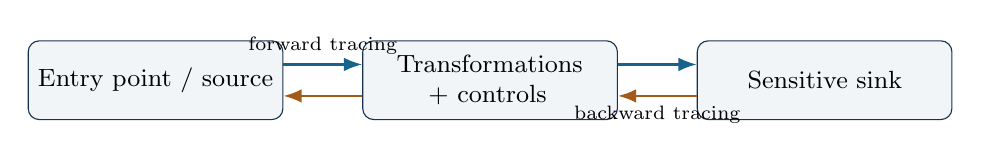
\begin{tikzpicture}[node distance=10mm, every node/.style={font=\small}, bx/.style={draw=navy,fill=papergray,rounded corners,minimum height=10mm,text width=3cm,align=center}, f/.style={-{Latex},thick,draw=azure},b/.style={-{Latex},thick,draw=warn}]
\node[bx](s){Entry point / source};\node[bx,right=of s](m){Transformations + controls};\node[bx,right=of m](k){Sensitive sink};
\draw[f] ([yshift=2mm]s.east)--node[above]{\scriptsize forward tracing}([yshift=2mm]m.west);
\draw[f] ([yshift=2mm]m.east)--([yshift=2mm]k.west);
\draw[b] ([yshift=-2mm]k.west)--node[below]{\scriptsize backward tracing}([yshift=-2mm]m.east);
\draw[b] ([yshift=-2mm]m.west)--([yshift=-2mm]s.east);
\end{tikzpicture}\caption{Forward tracing tests attacker influence; backward tracing tests sink reachability}\end{figure}

A forward trace asks whether untrusted input can reach relevant operations. A backward trace asks which caller contexts can reach a sensitive instruction and which guards dominate them. Complement these with a DG review for architectural invariants and error paths.

\chapter{Finding Validation and Exploitability Assessment}

\section{From query result to evidence-backed conclusion}

For every candidate, record the exact source node, confidence that it is attacker-controlled, propagation steps, decoding/encoding operations, guards, barrier semantics, reachable sink, runtime permissions, and production configuration. Use a minimal reproduction in an isolated fixture if the claim depends on runtime behavior. Preserve hypothetical assumptions distinctly from observed facts.

\begin{figure}[htbp]\centering
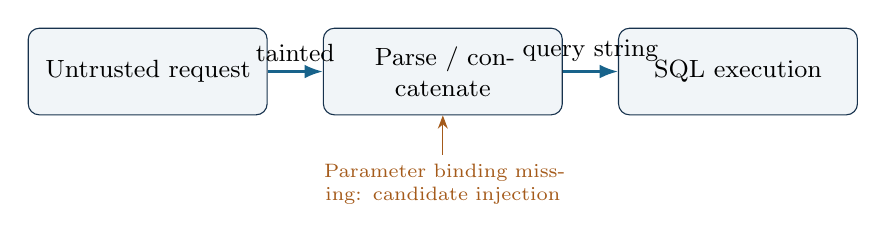
\begin{tikzpicture}[node distance=8mm and 7mm, every node/.style={font=\small}, v/.style={draw=navy,fill=papergray,rounded corners,text width=2.8cm,minimum height=11mm,align=center}, ar/.style={-{Latex},thick,draw=azure}]
\node[v](a){Untrusted request};\node[v,right=of a](b){Parse / concatenate};\node[v,right=of b](c){SQL execution};
\draw[ar](a)--node[above]{tainted}(b);\draw[ar](b)--node[above]{query string}(c);
\node[below=5mm of b,align=center,text width=3.7cm,font=\scriptsize\color{warn}](t){Parameter binding missing: candidate injection};
\draw[-{Stealth},draw=warn](t)--(b);
\end{tikzpicture}\caption{Hypothetical source-to-sink vulnerability trace}\end{figure}

\section{Triage evidence record}

\small
\setlength{\tabcolsep}{2pt}
\renewcommand{\arraystretch}{1.18}
\begin{longtable}{>{\raggedright\arraybackslash}p{0.22\linewidth}>{\raggedright\arraybackslash}p{0.73\linewidth}}
\toprule
\textbf{Element} & \textbf{Question and required record}\\
\midrule
\endfirsthead
\toprule
\textbf{Element} & \textbf{Question and required record}\\
\midrule
\endhead
Input & Can an external, lower-trust, or malicious principal influence the input?\\
Path & Which executable calls/branches propagate the input?\\
Context & Is the unsafe operation present in the assessed build/feature flag?\\
Controls & Does validation, prepared binding or authorization actually protect the sink?\\
Privilege & Which user/service identity and resources are available at the sink?\\
Impact & What confidentiality, integrity, or availability property could fail?\\
Reproduction & Is controlled, authorized testing possible and conclusive?\\
Conclusion & Confirmed, likely, not reproducible, false positive, or unverified; justify\\
\bottomrule
\end{longtable}
\normalsize

\section{Formalized confidence levels}

\begin{itemize}
\item \textbf{Observed:} complete validated path and reproducible security effect in an authorized fixture.
\item \textbf{Strong:} modeled path and code-level exploit preconditions validated; runtime reproduction unavailable.
\item \textbf{Moderate:} model and partial context support concern; material assumptions remain.
\item \textbf{Unresolved:} incomplete source, build coverage, sanitizer model, or deployment context.
\item \textbf{Rejected:} evidence invalidates critical premise; document exact source of model mismatch.
\end{itemize}

\section{Severity is not exploitability}

Keep CodeQL rule security severity separate from analyst confidence, exploit preconditions, network exposure, compensating controls and business criticality. An alert's high score does not demonstrate exploitation; conversely, a modest score may represent a critical business invariant in a privileged financial workflow. Avoid automatic multiplication of ordinal scales unless the enterprise risk framework specifies such a model.

\chapter{Vulnerability Assessment Catalog}

\section{Catalog usage and support labeling}

Each catalog entry is an \emph{assessment hypothesis}, not a claim that a specific repository contains a flaw. ``Builtin verified'' applies only when a specific official query ID has been checked in the current documentation; ``custom candidate'' describes a potential custom query but not a guaranteed implementation; ``manual-primary'' requires contextual inspection; ``unverified'' means coverage has not been established. CWE numbers identify plausible weakness families, not unique exploit proof.

\subsection{1. SQL injection}

\small
\setlength{\tabcolsep}{2pt}
\renewcommand{\arraystretch}{1.18}
\begin{longtable}{>{\raggedright\arraybackslash}p{0.26\linewidth}>{\raggedright\arraybackslash}p{0.69\linewidth}}
\toprule
\textbf{Assessment field} & \textbf{Evidence-based assessment instruction}\\
\midrule
\endfirsthead
\toprule
\textbf{Assessment field} & \textbf{Evidence-based assessment instruction}\\
\midrule
\endhead
\textbf{CWE and classification} & CWE-89; Implementation\\
\textbf{Root cause} & Untrusted bytes become part of executable SQL syntax\\
\textbf{Entry / source} & HTTP parameters / queue fields\\
\textbf{Sensitive sink} & Dynamic SQL execution\\
\textbf{CodeQL support} & Builtin verified for Python: 	exttt{py/sql-injection}; JavaScript: 	exttt{js/sql-injection}\\
\textbf{Validation and limits} & Prove input reaches SQL expression; inspect parameters, ORM raw query APIs and query construction. Analyze unmodeled frameworks, conditional guards and deployment specifics before deciding.\\
\textbf{Remediation} & Bind values through prepared statements; avoid user-defined SQL syntax\\
\textbf{Verification} & Assert malicious quote/comment characters remain data; test authorized and unauthorized queries\\
\textbf{Textbook grounding} & Dowd Ch.~8, 17--18; Bishop Ch.~31\\
\bottomrule
\end{longtable}
\normalsize

\subsection{2. OS command injection}

\small
\setlength{\tabcolsep}{2pt}
\renewcommand{\arraystretch}{1.18}
\begin{longtable}{>{\raggedright\arraybackslash}p{0.26\linewidth}>{\raggedright\arraybackslash}p{0.69\linewidth}}
\toprule
\textbf{Assessment field} & \textbf{Evidence-based assessment instruction}\\
\midrule
\endfirsthead
\toprule
\textbf{Assessment field} & \textbf{Evidence-based assessment instruction}\\
\midrule
\endhead
\textbf{CWE and classification} & CWE-78; Implementation\\
\textbf{Root cause} & User-influenced string is interpreted as shell syntax\\
\textbf{Entry / source} & Request data, filenames, environment\\
\textbf{Sensitive sink} & Shell invocation\\
\textbf{CodeQL support} & Builtin verified for JavaScript: 	exttt{js/command-line-injection}; other language coverage must be checked\\
\textbf{Validation and limits} & Trace string construction; confirm whether a shell is involved and which privileges execute. Analyze unmodeled frameworks, conditional guards and deployment specifics before deciding.\\
\textbf{Remediation} & Avoid shell; fixed executable with separated argument array; allowlist operations\\
\textbf{Verification} & Inputs containing metacharacters do not alter command structure\\
\textbf{Textbook grounding} & Dowd Ch.~8, 10, 18; Bishop Ch.~31\\
\bottomrule
\end{longtable}
\normalsize

\subsection{3. Cross-site scripting}

\small
\setlength{\tabcolsep}{2pt}
\renewcommand{\arraystretch}{1.18}
\begin{longtable}{>{\raggedright\arraybackslash}p{0.26\linewidth}>{\raggedright\arraybackslash}p{0.69\linewidth}}
\toprule
\textbf{Assessment field} & \textbf{Evidence-based assessment instruction}\\
\midrule
\endfirsthead
\toprule
\textbf{Assessment field} & \textbf{Evidence-based assessment instruction}\\
\midrule
\endhead
\textbf{CWE and classification} & CWE-79; Implementation / design\\
\textbf{Root cause} & Untrusted markup or script enters a browser execution context\\
\textbf{Entry / source} & Request, stored content\\
\textbf{Sensitive sink} & HTML/DOM insertion\\
\textbf{CodeQL support} & Custom candidate; verify installed built-in query per target language\\
\textbf{Validation and limits} & Inspect browser context, response content type, templating autoescaping and CSP. Analyze unmodeled frameworks, conditional guards and deployment specifics before deciding.\\
\textbf{Remediation} & Context-sensitive encoding, safe DOM APIs, sanitization when rich HTML is required\\
\textbf{Verification} & Browser test with inert canary script in safe fixture\\
\textbf{Textbook grounding} & Dowd Ch.~17--18; Bishop Ch.~14, 31\\
\bottomrule
\end{longtable}
\normalsize

\subsection{4. Path traversal}

\small
\setlength{\tabcolsep}{2pt}
\renewcommand{\arraystretch}{1.18}
\begin{longtable}{>{\raggedright\arraybackslash}p{0.26\linewidth}>{\raggedright\arraybackslash}p{0.69\linewidth}}
\toprule
\textbf{Assessment field} & \textbf{Evidence-based assessment instruction}\\
\midrule
\endfirsthead
\toprule
\textbf{Assessment field} & \textbf{Evidence-based assessment instruction}\\
\midrule
\endhead
\textbf{CWE and classification} & CWE-22; Implementation\\
\textbf{Root cause} & Untrusted path escapes intended directory\\
\textbf{Entry / source} & URL, archive name, filename\\
\textbf{Sensitive sink} & Filesystem open/create/delete\\
\textbf{CodeQL support} & Custom candidate; query for remote-to-file paths shown in Ch.~5\\
\textbf{Validation and limits} & Resolve real paths and links; inspect containment race and permission boundaries. Analyze unmodeled frameworks, conditional guards and deployment specifics before deciding.\\
\textbf{Remediation} & Use fixed base, canonical containment, opaque IDs and least-privileged filesystem access\\
\textbf{Verification} & Traversal and encoded variants are denied; symlink tests pass\\
\textbf{Textbook grounding} & Dowd Ch.~8--9; Bishop Ch.~16, 31\\
\bottomrule
\end{longtable}
\normalsize

\subsection{5. Server-side request forgery}

\small
\setlength{\tabcolsep}{2pt}
\renewcommand{\arraystretch}{1.18}
\begin{longtable}{>{\raggedright\arraybackslash}p{0.26\linewidth}>{\raggedright\arraybackslash}p{0.69\linewidth}}
\toprule
\textbf{Assessment field} & \textbf{Evidence-based assessment instruction}\\
\midrule
\endfirsthead
\toprule
\textbf{Assessment field} & \textbf{Evidence-based assessment instruction}\\
\midrule
\endhead
\textbf{CWE and classification} & CWE-918; Implementation / design\\
\textbf{Root cause} & Attacker chooses server-side connection target\\
\textbf{Entry / source} & URL, redirect target, webhook\\
\textbf{Sensitive sink} & Outbound HTTP/DNS\\
\textbf{CodeQL support} & Custom candidate; inspect verified language-specific builtins\\
\textbf{Validation and limits} & Assess DNS rebinding, redirects, address parsing, network egress and metadata access. Analyze unmodeled frameworks, conditional guards and deployment specifics before deciding.\\
\textbf{Remediation} & Allowlist trusted endpoints; enforce egress controls and redirect policy\\
\textbf{Verification} & Internal-address and redirect tests blocked in isolated network\\
\textbf{Textbook grounding} & Dowd Ch.~16--17; Bishop Ch.~14, 28\\
\bottomrule
\end{longtable}
\normalsize

\subsection{6. XML external entities}

\small
\setlength{\tabcolsep}{2pt}
\renewcommand{\arraystretch}{1.18}
\begin{longtable}{>{\raggedright\arraybackslash}p{0.26\linewidth}>{\raggedright\arraybackslash}p{0.69\linewidth}}
\toprule
\textbf{Assessment field} & \textbf{Evidence-based assessment instruction}\\
\midrule
\endfirsthead
\toprule
\textbf{Assessment field} & \textbf{Evidence-based assessment instruction}\\
\midrule
\endhead
\textbf{CWE and classification} & CWE-611; Implementation / configuration\\
\textbf{Root cause} & Parser loads external entities or network resources\\
\textbf{Entry / source} & Untrusted XML document\\
\textbf{Sensitive sink} & XML parser/entity resolution\\
\textbf{CodeQL support} & Custom candidate; parser configuration is library-dependent\\
\textbf{Validation and limits} & Inspect DTD/entity flags and recursive parsing, unsafe document formats. Analyze unmodeled frameworks, conditional guards and deployment specifics before deciding.\\
\textbf{Remediation} & Disable external entities/DTDs and resource resolution\\
\textbf{Verification} & Entity payload yields error/no remote request in sandbox\\
\textbf{Textbook grounding} & Dowd Ch.~16, 18; Bishop Ch.~31\\
\bottomrule
\end{longtable}
\normalsize

\subsection{7. Unsafe deserialization}

\small
\setlength{\tabcolsep}{2pt}
\renewcommand{\arraystretch}{1.18}
\begin{longtable}{>{\raggedright\arraybackslash}p{0.26\linewidth}>{\raggedright\arraybackslash}p{0.69\linewidth}}
\toprule
\textbf{Assessment field} & \textbf{Evidence-based assessment instruction}\\
\midrule
\endfirsthead
\toprule
\textbf{Assessment field} & \textbf{Evidence-based assessment instruction}\\
\midrule
\endhead
\textbf{CWE and classification} & CWE-502; Implementation / design\\
\textbf{Root cause} & Untrusted serialized content controls object construction\\
\textbf{Entry / source} & Network/session/queue blobs\\
\textbf{Sensitive sink} & Deserializer gadget execution\\
\textbf{CodeQL support} & Custom candidate; framework-specific models required\\
\textbf{Validation and limits} & Verify deserializer semantics, allowlists, integrity and type resolution. Analyze unmodeled frameworks, conditional guards and deployment specifics before deciding.\\
\textbf{Remediation} & Use inert data formats, typed schemas and authenticated messages\\
\textbf{Verification} & Fixture with disallowed types and tampered bytes rejected\\
\textbf{Textbook grounding} & Dowd Ch.~2, 16; Bishop Ch.~14, 31\\
\bottomrule
\end{longtable}
\normalsize

\subsection{8. Dynamic code injection}

\small
\setlength{\tabcolsep}{2pt}
\renewcommand{\arraystretch}{1.18}
\begin{longtable}{>{\raggedright\arraybackslash}p{0.26\linewidth}>{\raggedright\arraybackslash}p{0.69\linewidth}}
\toprule
\textbf{Assessment field} & \textbf{Evidence-based assessment instruction}\\
\midrule
\endfirsthead
\toprule
\textbf{Assessment field} & \textbf{Evidence-based assessment instruction}\\
\midrule
\endhead
\textbf{CWE and classification} & CWE-94; Implementation\\
\textbf{Root cause} & Untrusted bytes reach language evaluator\\
\textbf{Entry / source} & User expressions / templates\\
\textbf{Sensitive sink} & eval/exec / dynamic compilation\\
\textbf{CodeQL support} & Builtin verified Python: 	exttt{py/code-injection}; JavaScript: 	exttt{js/code-injection}\\
\textbf{Validation and limits} & Check reachability, evaluator grammar, escaping and privileges. Analyze unmodeled frameworks, conditional guards and deployment specifics before deciding.\\
\textbf{Remediation} & Remove evaluator; replace with constrained parser/interpreter\\
\textbf{Verification} & Untrusted expressions never execute code or change globals\\
\textbf{Textbook grounding} & Dowd Ch.~17--18; Bishop Ch.~31\\
\bottomrule
\end{longtable}
\normalsize

\subsection{9. Buffer overflow}

\small
\setlength{\tabcolsep}{2pt}
\renewcommand{\arraystretch}{1.18}
\begin{longtable}{>{\raggedright\arraybackslash}p{0.26\linewidth}>{\raggedright\arraybackslash}p{0.69\linewidth}}
\toprule
\textbf{Assessment field} & \textbf{Evidence-based assessment instruction}\\
\midrule
\endfirsthead
\toprule
\textbf{Assessment field} & \textbf{Evidence-based assessment instruction}\\
\midrule
\endhead
\textbf{CWE and classification} & CWE-120; Implementation\\
\textbf{Root cause} & Writes exceed destination memory boundary\\
\textbf{Entry / source} & Network payload / size fields\\
\textbf{Sensitive sink} & Copy/write to fixed buffer\\
\textbf{CodeQL support} & Custom candidate; C/C++ built-in coverage must be checked\\
\textbf{Validation and limits} & Trace size units, null termination, indexes, allocator sizes. Analyze unmodeled frameworks, conditional guards and deployment specifics before deciding.\\
\textbf{Remediation} & Use bounded abstractions and checked lengths\\
\textbf{Verification} & Boundary-length and fuzz tests with sanitizers\\
\textbf{Textbook grounding} & Dowd Ch.~5, 7--8; Bishop Ch.~31\\
\bottomrule
\end{longtable}
\normalsize

\subsection{10. Integer wrap/truncation}

\small
\setlength{\tabcolsep}{2pt}
\renewcommand{\arraystretch}{1.18}
\begin{longtable}{>{\raggedright\arraybackslash}p{0.26\linewidth}>{\raggedright\arraybackslash}p{0.69\linewidth}}
\toprule
\textbf{Assessment field} & \textbf{Evidence-based assessment instruction}\\
\midrule
\endfirsthead
\toprule
\textbf{Assessment field} & \textbf{Evidence-based assessment instruction}\\
\midrule
\endhead
\textbf{CWE and classification} & CWE-190 / CWE-197; Implementation\\
\textbf{Root cause} & Arithmetic and conversions violate allocation or length invariant\\
\textbf{Entry / source} & File sizes / network length\\
\textbf{Sensitive sink} & Allocation, index, loop bounds\\
\textbf{CodeQL support} & Custom candidate; no blanket built-in assertion\\
\textbf{Validation and limits} & Trace signedness, promotions, upper bounds and wraparound effects. Analyze unmodeled frameworks, conditional guards and deployment specifics before deciding.\\
\textbf{Remediation} & Checked arithmetic and constrained types\\
\textbf{Verification} & Min/max, negative, and near-overflow tests\\
\textbf{Textbook grounding} & Dowd Ch.~6--7; Bishop Ch.~31\\
\bottomrule
\end{longtable}
\normalsize

\subsection{11. Use-after-free/double-free}

\small
\setlength{\tabcolsep}{2pt}
\renewcommand{\arraystretch}{1.18}
\begin{longtable}{>{\raggedright\arraybackslash}p{0.26\linewidth}>{\raggedright\arraybackslash}p{0.69\linewidth}}
\toprule
\textbf{Assessment field} & \textbf{Evidence-based assessment instruction}\\
\midrule
\endfirsthead
\toprule
\textbf{Assessment field} & \textbf{Evidence-based assessment instruction}\\
\midrule
\endhead
\textbf{CWE and classification} & CWE-416 / CWE-415; Implementation\\
\textbf{Root cause} & Object lifetime violated before memory access or release\\
\textbf{Entry / source} & Complex state / error paths\\
\textbf{Sensitive sink} & free/delete/dereference\\
\textbf{CodeQL support} & Custom candidate; verify available C/C++ query coverage\\
\textbf{Validation and limits} & Trace ownership, aliases, exception cleanup, concurrent operations. Analyze unmodeled frameworks, conditional guards and deployment specifics before deciding.\\
\textbf{Remediation} & RAII/ownership types; null/disable handles after release\\
\textbf{Verification} & ASan tests and lifetime-focused unit cases\\
\textbf{Textbook grounding} & Dowd Ch.~5, 7; Bishop Ch.~31\\
\bottomrule
\end{longtable}
\normalsize

\subsection{12. Race condition / TOCTOU}

\small
\setlength{\tabcolsep}{2pt}
\renewcommand{\arraystretch}{1.18}
\begin{longtable}{>{\raggedright\arraybackslash}p{0.26\linewidth}>{\raggedright\arraybackslash}p{0.69\linewidth}}
\toprule
\textbf{Assessment field} & \textbf{Evidence-based assessment instruction}\\
\midrule
\endfirsthead
\toprule
\textbf{Assessment field} & \textbf{Evidence-based assessment instruction}\\
\midrule
\endhead
\textbf{CWE and classification} & CWE-362 / CWE-367; Implementation / design\\
\textbf{Root cause} & State changes between validation and sensitive operation\\
\textbf{Entry / source} & Concurrent requests / filesystem\\
\textbf{Sensitive sink} & check-then-use / shared mutation\\
\textbf{CodeQL support} & Manual-primary; limited pattern-based query potential\\
\textbf{Validation and limits} & Reconstruct interleavings and atomicity/locking guarantees. Analyze unmodeled frameworks, conditional guards and deployment specifics before deciding.\\
\textbf{Remediation} & Atomic API, lock or transaction, descriptor-based checks\\
\textbf{Verification} & Repeated concurrency/interleaving harness tests\\
\textbf{Textbook grounding} & Dowd Ch.~9, 13; Bishop Ch.~7, 31\\
\bottomrule
\end{longtable}
\normalsize

\subsection{13. Insecure temporary files}

\small
\setlength{\tabcolsep}{2pt}
\renewcommand{\arraystretch}{1.18}
\begin{longtable}{>{\raggedright\arraybackslash}p{0.26\linewidth}>{\raggedright\arraybackslash}p{0.69\linewidth}}
\toprule
\textbf{Assessment field} & \textbf{Evidence-based assessment instruction}\\
\midrule
\endfirsthead
\toprule
\textbf{Assessment field} & \textbf{Evidence-based assessment instruction}\\
\midrule
\endhead
\textbf{CWE and classification} & CWE-377; Implementation / operational\\
\textbf{Root cause} & Predictable or shared temporary file allows substitution\\
\textbf{Entry / source} & Temporary namespace\\
\textbf{Sensitive sink} & create/open/temp writer\\
\textbf{CodeQL support} & Custom candidate; library-specific APIs\\
\textbf{Validation and limits} & Check create flags, symlinks, ownership, mode and cleanup. Analyze unmodeled frameworks, conditional guards and deployment specifics before deciding.\\
\textbf{Remediation} & Use secure atomic tempfile API with restrictive modes\\
\textbf{Verification} & Concurrent reuse and symlink tests isolated\\
\textbf{Textbook grounding} & Dowd Ch.~9; Bishop Ch.~16, 31\\
\bottomrule
\end{longtable}
\normalsize

\subsection{14. Improper authentication}

\small
\setlength{\tabcolsep}{2pt}
\renewcommand{\arraystretch}{1.18}
\begin{longtable}{>{\raggedright\arraybackslash}p{0.26\linewidth}>{\raggedright\arraybackslash}p{0.69\linewidth}}
\toprule
\textbf{Assessment field} & \textbf{Evidence-based assessment instruction}\\
\midrule
\endfirsthead
\toprule
\textbf{Assessment field} & \textbf{Evidence-based assessment instruction}\\
\midrule
\endhead
\textbf{CWE and classification} & CWE-287; Design / implementation\\
\textbf{Root cause} & Identity validation bypassed, absent or inconsistent\\
\textbf{Entry / source} & Tokens / credentials\\
\textbf{Sensitive sink} & Protected service entry\\
\textbf{CodeQL support} & Manual-primary for protocol correctness; custom candidate for known APIs\\
\textbf{Validation and limits} & Examine identity binding, token audience, expiry, MFA and session state. Analyze unmodeled frameworks, conditional guards and deployment specifics before deciding.\\
\textbf{Remediation} & Centralized, complete verification with negative tests\\
\textbf{Verification} & Malformed, expired, wrong-audience, and forged token cases denied\\
\textbf{Textbook grounding} & Dowd Ch.~2, 17; Bishop Ch.~12, 15\\
\bottomrule
\end{longtable}
\normalsize

\subsection{15. Broken authorization}

\small
\setlength{\tabcolsep}{2pt}
\renewcommand{\arraystretch}{1.18}
\begin{longtable}{>{\raggedright\arraybackslash}p{0.26\linewidth}>{\raggedright\arraybackslash}p{0.69\linewidth}}
\toprule
\textbf{Assessment field} & \textbf{Evidence-based assessment instruction}\\
\midrule
\endfirsthead
\toprule
\textbf{Assessment field} & \textbf{Evidence-based assessment instruction}\\
\midrule
\endhead
\textbf{CWE and classification} & CWE-862 / CWE-639; Design\\
\textbf{Root cause} & Missing object/action-level permission enforcement\\
\textbf{Entry / source} & Object identifiers, roles\\
\textbf{Sensitive sink} & Data retrieval, state change\\
\textbf{CodeQL support} & Manual-primary; project-specific query possible\\
\textbf{Validation and limits} & Check owner/tenant relation at each sensitive operation; no client-supplied trust. Analyze unmodeled frameworks, conditional guards and deployment specifics before deciding.\\
\textbf{Remediation} & Server-side policy enforcement at object boundary\\
\textbf{Verification} & Cross-tenant and role matrix must deny forbidden combinations\\
\textbf{Textbook grounding} & Dowd Ch.~2, 17; Bishop Ch.~14, 16\\
\bottomrule
\end{longtable}
\normalsize

\subsection{16. Weak cryptography / key misuse}

\small
\setlength{\tabcolsep}{2pt}
\renewcommand{\arraystretch}{1.18}
\begin{longtable}{>{\raggedright\arraybackslash}p{0.26\linewidth}>{\raggedright\arraybackslash}p{0.69\linewidth}}
\toprule
\textbf{Assessment field} & \textbf{Evidence-based assessment instruction}\\
\midrule
\endfirsthead
\toprule
\textbf{Assessment field} & \textbf{Evidence-based assessment instruction}\\
\midrule
\endhead
\textbf{CWE and classification} & CWE-327 / CWE-798; Design / implementation\\
\textbf{Root cause} & Sensitive data protected by weak cipher, key reuse or exposed secret\\
\textbf{Entry / source} & Configuration, static strings\\
\textbf{Sensitive sink} & Crypto primitive / key storage\\
\textbf{CodeQL support} & Custom candidate; verify language-specific builtin cryptographic rules\\
\textbf{Validation and limits} & Examine algorithm mode, nonce lifecycle, randomness, key rotation and threat model. Analyze unmodeled frameworks, conditional guards and deployment specifics before deciding.\\
\textbf{Remediation} & Modern authenticated encryption and managed key lifecycle\\
\textbf{Verification} & Known-answer and key-rotation tests; review config\\
\textbf{Textbook grounding} & Dowd Ch.~2, 17; Bishop Ch.~8--13\\
\bottomrule
\end{longtable}
\normalsize

\subsection{17. Sensitive data exposure}

\small
\setlength{\tabcolsep}{2pt}
\renewcommand{\arraystretch}{1.18}
\begin{longtable}{>{\raggedright\arraybackslash}p{0.26\linewidth}>{\raggedright\arraybackslash}p{0.69\linewidth}}
\toprule
\textbf{Assessment field} & \textbf{Evidence-based assessment instruction}\\
\midrule
\endfirsthead
\toprule
\textbf{Assessment field} & \textbf{Evidence-based assessment instruction}\\
\midrule
\endhead
\textbf{CWE and classification} & CWE-200; Design / implementation\\
\textbf{Root cause} & Sensitive information reaches logs or external consumers\\
\textbf{Entry / source} & PII, tokens, private records\\
\textbf{Sensitive sink} & Logs, errors, responses\\
\textbf{CodeQL support} & Custom candidate; project-specific sensitivity models\\
\textbf{Validation and limits} & Trace classified data and serialization/redaction. Analyze unmodeled frameworks, conditional guards and deployment specifics before deciding.\\
\textbf{Remediation} & Minimize retention, redact, scope outputs, deny unrelated access\\
\textbf{Verification} & Canary secrets absent from logs/errors under failure paths\\
\textbf{Textbook grounding} & Dowd Ch.~1--3, 17; Bishop Ch.~1, 17\\
\bottomrule
\end{longtable}
\normalsize

\subsection{18. Hardcoded credentials}

\small
\setlength{\tabcolsep}{2pt}
\renewcommand{\arraystretch}{1.18}
\begin{longtable}{>{\raggedright\arraybackslash}p{0.26\linewidth}>{\raggedright\arraybackslash}p{0.69\linewidth}}
\toprule
\textbf{Assessment field} & \textbf{Evidence-based assessment instruction}\\
\midrule
\endfirsthead
\toprule
\textbf{Assessment field} & \textbf{Evidence-based assessment instruction}\\
\midrule
\endhead
\textbf{CWE and classification} & CWE-798; Implementation / operational\\
\textbf{Root cause} & Embedded credential grants access outside secret lifecycle\\
\textbf{Entry / source} & Literal tokens / connection strings\\
\textbf{Sensitive sink} & Authentication configuration\\
\textbf{CodeQL support} & Custom candidate in CodeQL; dedicated secret scanning separate\\
\textbf{Validation and limits} & Confirm literal is functional secret, validity/rotation, exposure. Analyze unmodeled frameworks, conditional guards and deployment specifics before deciding.\\
\textbf{Remediation} & Use secret manager and rotation; revoke exposed credentials\\
\textbf{Verification} & Revocation verified, no embedded secret; separate secret scan\\
\textbf{Textbook grounding} & Dowd Ch.~1, 3; Bishop Ch.~14, 31\\
\bottomrule
\end{longtable}
\normalsize

\subsection{19. Resource exhaustion}

\small
\setlength{\tabcolsep}{2pt}
\renewcommand{\arraystretch}{1.18}
\begin{longtable}{>{\raggedright\arraybackslash}p{0.26\linewidth}>{\raggedright\arraybackslash}p{0.69\linewidth}}
\toprule
\textbf{Assessment field} & \textbf{Evidence-based assessment instruction}\\
\midrule
\endfirsthead
\toprule
\textbf{Assessment field} & \textbf{Evidence-based assessment instruction}\\
\midrule
\endhead
\textbf{CWE and classification} & CWE-400; Design / implementation\\
\textbf{Root cause} & Unbounded work/memory allocation exhausts service\\
\textbf{Entry / source} & Length, iteration, regex input\\
\textbf{Sensitive sink} & Loops, allocators, regex\\
\textbf{CodeQL support} & Manual-primary; pattern queries may aid candidates\\
\textbf{Validation and limits} & Model worst-case cost, quotas and concurrency. Analyze unmodeled frameworks, conditional guards and deployment specifics before deciding.\\
\textbf{Remediation} & Bound input/time/memory; rate and concurrency controls\\
\textbf{Verification} & Load/fuzz thresholds and enforced deadlines\\
\textbf{Textbook grounding} & Dowd Ch.~5--7, 13, 17; Bishop Ch.~7, 31\\
\bottomrule
\end{longtable}
\normalsize

\subsection{20. Improper error handling}

\small
\setlength{\tabcolsep}{2pt}
\renewcommand{\arraystretch}{1.18}
\begin{longtable}{>{\raggedright\arraybackslash}p{0.26\linewidth}>{\raggedright\arraybackslash}p{0.69\linewidth}}
\toprule
\textbf{Assessment field} & \textbf{Evidence-based assessment instruction}\\
\midrule
\endfirsthead
\toprule
\textbf{Assessment field} & \textbf{Evidence-based assessment instruction}\\
\midrule
\endhead
\textbf{CWE and classification} & CWE-755; Implementation / design\\
\textbf{Root cause} & Error path bypasses policy or leaves invalid security state\\
\textbf{Entry / source} & Exceptions, dependency failure\\
\textbf{Sensitive sink} & catch/finally/fallback\\
\textbf{CodeQL support} & Custom candidate; manual failure-injection needed\\
\textbf{Validation and limits} & Review error rollback, default decision and cleanup. Analyze unmodeled frameworks, conditional guards and deployment specifics before deciding.\\
\textbf{Remediation} & Fail closed, transactional rollback, safe logging\\
\textbf{Verification} & Fault injection confirms safe state transitions\\
\textbf{Textbook grounding} & Dowd Ch.~1, 7, 13; Bishop Ch.~14, 31\\
\bottomrule
\end{longtable}
\normalsize

\subsection{21. Unsafe dependencies and APIs}

\small
\setlength{\tabcolsep}{2pt}
\renewcommand{\arraystretch}{1.18}
\begin{longtable}{>{\raggedright\arraybackslash}p{0.26\linewidth}>{\raggedright\arraybackslash}p{0.69\linewidth}}
\toprule
\textbf{Assessment field} & \textbf{Evidence-based assessment instruction}\\
\midrule
\endfirsthead
\toprule
\textbf{Assessment field} & \textbf{Evidence-based assessment instruction}\\
\midrule
\endhead
\textbf{CWE and classification} & CWE-1104; Operational / implementation\\
\textbf{Root cause} & Outdated or misused dependency exposes known weakness\\
\textbf{Entry / source} & Manifest / transitive library\\
\textbf{Sensitive sink} & Vulnerable dependency invocation\\
\textbf{CodeQL support} & Manual-primary plus SCA; CodeQL may detect unsafe usage patterns\\
\textbf{Validation and limits} & Correlate affected version, exploit path and runtime exposure. Analyze unmodeled frameworks, conditional guards and deployment specifics before deciding.\\
\textbf{Remediation} & Upgrade/remove, switch safer API; verify reachable impact\\
\textbf{Verification} & Build + regression + dependency advisory evidence\\
\textbf{Textbook grounding} & Dowd Ch.~3--4; Bishop Ch.~19--20\\
\bottomrule
\end{longtable}
\normalsize

\chapter{Language-Specific Source Code Assessment}

\section{Language risk profiles and coverage caveats}

\small
\setlength{\tabcolsep}{2pt}
\renewcommand{\arraystretch}{1.18}
\begin{longtable}{>{\raggedright\arraybackslash}p{0.13\linewidth}>{\raggedright\arraybackslash}p{0.27\linewidth}>{\raggedright\arraybackslash}p{0.27\linewidth}>{\raggedright\arraybackslash}p{0.28\linewidth}}
\toprule
\textbf{Language} & \textbf{Risk surface} & \textbf{Review priority} & \textbf{Validation note}\\
\midrule
\endfirsthead
\toprule
\textbf{Language} & \textbf{Risk surface} & \textbf{Review priority} & \textbf{Validation note}\\
\midrule
\endhead
C / C++ & Pointer arithmetic; allocators; signedness; lifetimes; C/C++ header and build configurations & Memory bounds, format strings, overflow, TOCTOU, casting, macro-defined behavior & Inspect compiler flags, macro branches, allocation-unit invariants and sanitizer fixtures.\\
C\# & ASP.NET Core model binding; EF/SQL; claims and authorization attributes; deserializers & SQL/command injection, SSRF, authorization gaps, unsafe reflection & Review dependency injection, endpoint policy, EF raw SQL parameter binding and background job roles.\\
Java / Kotlin & Servlet/Spring route handling; JDBC; XML; reflection; object deserialization & SQL injection, XXE, SSRF, insecure Java deserialization & Kotlin requires build-capable extraction; check Spring Security filters and method guards.\\
JavaScript / TypeScript & Node.js child processes; templating; prototype behavior; browser DOM & Injection, XSS, prototype pollution, SSRF, insecure workflow expressions & Differentiate browser/server sinks, bundled and generated code, framework escaping.\\
Python & Flask/FastAPI/Django; SQLAlchemy; subprocess; pickle; os.open & SQL/code injection, dynamic exec, path traversal, SSRF & Inspect middleware, application routes and dependency wrappers not modeled.\\
Go & net/http, database/sql, os/exec, HTML templates, goroutines & Command/SQL injection, request handling, unsafe path use and races & Check goroutine sharing, policy checks and runtime race detector separately.\\
Ruby & Rails strong parameters, ActiveRecord raw SQL, ERB & SQL injection, mass assignment, command injection, auth gaps & Trace Rails conventions and gems; analyze implicit sources/sinks.\\
Rust & unsafe blocks, FFI, interior mutability, unsafe serialization & Unsafe memory, FFI boundary, overflow and logic vulnerabilities & CodeQL support evolves; complement with compiler/lint and unsafe reviews.\\
Swift & Foundation URL networking, filesystem, bridging, crypto APIs & Privacy, unsafe URL handling, insecure storage, logic defects & Validate platform-specific APIs, entitlements, iOS/macOS build extraction.\\
GitHub Actions & Expression contexts, permissions, third-party actions, artifacts & Command injection and supply-chain privilege misuse & Treat workflow configuration as code; verify event model and fork permissions.\\
\bottomrule
\end{longtable}
\normalsize

\section{Python: SQL injection and safe parameter binding}

\begin{lstlisting}[caption={Python sqlite3: unsafe concatenation versus parameter binding},language=Python]
def lookup_bad(conn, label):
    sql = "SELECT id FROM inventory WHERE label = '" + label + "'"
    return conn.execute(sql).fetchall()

def lookup_good(conn, label):
    return conn.execute(
        "SELECT id FROM inventory WHERE label = ?", (label,)
    ).fetchall()
\end{lstlisting}

\srcM\ Official query-help identifies \texttt{py/sql-injection} and uses CWE-89. \srcR\ Test with quote-containing input and verify unchanged SQL semantics, not merely absence of alerts. Bind values only; query identifiers require separate allowlist logic.

\section{JavaScript: shell evaluation}

\begin{lstlisting}[caption={Node.js: shell string versus separated arguments}]
const cp = require('node:child_process');
function badCount(filename) {
  cp.execSync('wc -l ' + filename); // shell interprets metacharacters
}
function goodCount(filename) {
  return cp.execFileSync('wc', ['-l', '--', filename],
                         {shell: false});
}
\end{lstlisting}

\srcM\ Official \texttt{js/command-line-injection} covers command strings from untrusted values. Even argument-array APIs need safe option handling (\texttt{--} is command-specific) and appropriate file authorization. For general portability prefer an in-process file-reading API if the operation is simple.

\section{C: buffer size verification}

\begin{lstlisting}[caption={C11: guarded copy with explicit capacity contract},language=C]
#include <stddef.h>
#include <string.h>
int copy_label(char *dst, size_t capacity, const char *src) {
    size_t len = strlen(src);
    if (capacity == 0 || len >= capacity) return -1;
    memcpy(dst, src, len + 1);
    return 0;
}
\end{lstlisting}

The snippet assumes \texttt{src} is valid and NUL-terminated and \texttt{dst} points to a real allocation of at least \texttt{capacity} bytes; these remain separate preconditions. For untrusted non-terminated buffers use length-aware input functions. \srcD\ Dowd Chapters 5--8 give the underlying memory, arithmetic and string-auditing rationale.

\section{Java: prepared statements}

\begin{lstlisting}[caption={Java: JDBC prepared statement (context assumes valid connection)},language=Java]
String sql = "SELECT id FROM inventory WHERE label = ?";
try (PreparedStatement ps = conn.prepareStatement(sql)) {
    ps.setString(1, label);
    try (ResultSet rs = ps.executeQuery()) {
        while (rs.next()) { /* process rows */ }
    }
}
\end{lstlisting}

\section{C\#: parameterized database command}

\begin{lstlisting}[caption={C sharp: parameterized ADO.NET (provider-specific details apply)}]
using var cmd = connection.CreateCommand();
cmd.CommandText = "SELECT Id FROM Inventory WHERE Label = @label";
var p = cmd.CreateParameter();
p.ParameterName = "@label";
p.Value = label;
cmd.Parameters.Add(p);
using var reader = cmd.ExecuteReader();
\end{lstlisting}

\section{Go: argument binding and timeouts}

\begin{lstlisting}[caption={Go: context-bounded parameterized query skeleton}]
ctx, cancel := context.WithTimeout(r.Context(), 2*time.Second)
defer cancel()
row := db.QueryRowContext(ctx,
    "SELECT id FROM inventory WHERE label = ?", label)
_ = row // inspect driver placeholder dialect and scan error
\end{lstlisting}

Go placeholders vary by SQL driver (for example, PostgreSQL generally uses numbered placeholders); this snippet is illustrative and does not compile standalone without imports/variables. A correct full project should test cancellation, denied object ownership, and actual driver behavior.

\chapter{GitHub Code Scanning and CodeQL Integration}

\section{Platform setup and event coverage}

\srcM\ GitHub code scanning integrates CodeQL analysis with repository alerts and pull-request annotations. The documentation distinguishes default setup from advanced setup. Workflows should scan the default branch, relevant pull requests, and a periodic schedule if required for newly added queries. Confirm policies for forks, changed branches, default setup visibility and generated-code behavior before claiming complete prevention.

\begin{lstlisting}[caption={Illustrative GitHub Actions advanced setup (adapt to repo)}]
name: CodeQL assessment
on:
  push:
    branches: [main]
  pull_request:
    branches: [main]
  schedule:
    - cron: '17 3 * * 1'
permissions:
  contents: read
  security-events: write
jobs:
  analyze:
    runs-on: ubuntu-latest
    strategy:
      fail-fast: false
      matrix:
        include:
          - language: python
            build-mode: none
          - language: javascript-typescript
            build-mode: none
    steps:
      - uses: actions/checkout@v4
      - uses: github/codeql-action/init@v4
        with:
          languages: ${{ matrix.language }}
          build-mode: ${{ matrix.build-mode }}
          queries: security-extended
      - uses: github/codeql-action/analyze@v4
\end{lstlisting}

\limt\ This workflow is an example, not an executed CI run. For compiled language repositories use a supported build mode, configure build steps and matrix entries appropriately. Restrict workflow token permissions, pin trusted action revisions where organization policy requires it, and verify enterprise runner access. Version \texttt{@v4} corresponds to official current documentation reviewed on 2026-10-16; subsequent releases may change requirements.

\section{Security gate semantics}

A PR gate should assert the actual security property required: the CodeQL job analyzed the proposed fix commit in a branch/PR context, checks passed, and relevant alert thresholds are enforced. A scan configured only for push to \texttt{main} cannot prove the fix was scanned \emph{before} merge. Required status checks do not automatically establish that every language or query suite executed.

\section{Product boundary: scanning versus secrets and dependencies}

CodeQL analyzes source code via static queries; GitHub secret scanning identifies exposed secret patterns and other supported detectors; Dependabot detects vulnerable dependencies using advisory and dependency graphs. These capabilities produce separate evidence streams. A vulnerable dependency is not necessarily exploitable, and a valid leaked credential may not be detectable by CodeQL.

\section{Query-suite configuration and upgrades}

Official default queries prioritize precision; \texttt{security-extended} adds additional queries and potential review burden. Maintain a baseline query manifest; pin and periodically refresh custom packs, run fixture tests on upgrades, monitor query changes, and document changes in reported counts. Do not interpret a sudden alert decrease as a pure remediation success without ruling out analysis coverage changes.

\chapter{Enterprise Repository-Wide CodeQL Audit}

\section{Scope, evidence sources and architecture}

Start from authoritative repository inventory and security ownership, not only repositories currently producing alerts. Join repo metadata, technology inventory, CodeQL configuration, workflow runs, alert state, branch protection, exceptions, and criticality. Organization-level alert APIs list default-branch alerts for eligible repositories and are \emph{not} a complete inventory of repository coverage; obtain separate repository and analysis metadata.

\begin{figure}[htbp]\centering
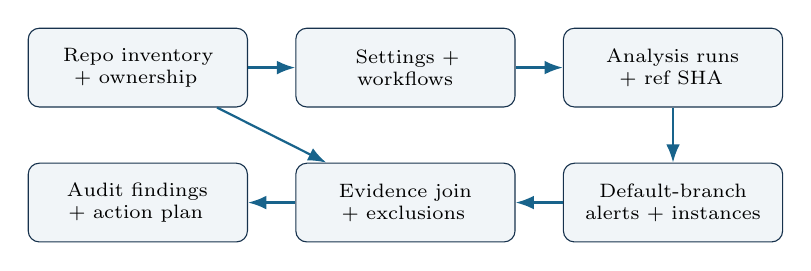
\begin{tikzpicture}[node distance=7mm and 6mm,every node/.style={font=\scriptsize},bx/.style={draw=navy,fill=papergray,rounded corners,text width=2.55cm,align=center,minimum height=10mm},ar/.style={-{Latex},thick,draw=azure}]
\node[bx](inv){Repo inventory + ownership};\node[bx,right=of inv](config){Settings + workflows};\node[bx,right=of config](run){Analysis runs + ref SHA};\node[bx,below=of run](alerts){Default-branch alerts + instances};\node[bx,left=of alerts](join){Evidence join + exclusions};\node[bx,left=of join](report){Audit findings + action plan};
\draw[ar](inv)--(config);\draw[ar](config)--(run);\draw[ar](run)--(alerts);\draw[ar](alerts)--(join);\draw[ar](join)--(report);\draw[ar](inv)--(join);
\end{tikzpicture}\caption{Enterprise audit evidence join across repositories, configuration, runs, and alerts}\end{figure}

\section{REST API collection pattern}

\srcM\ GitHub REST API version \texttt{2026-03-10} documents an organization-level CodeQL alert endpoint, with owner/security-manager and appropriate code-scanning alert permissions. Result content includes state, rule ID, tool, locations, timestamps and dismissal metadata when applicable. Permission errors, pagination, rate limits, and the default-branch limitation must be reported as coverage defects, not silently treated as zero findings.

\begin{lstlisting}[caption={Organization-level CodeQL alert extraction example},language=bash]
# Using GitHub CLI with an authorized token and required scopes.
# Keep org identifier in your local environment.
ORG="YOUR-ORG"
gh api --paginate \
  -H "X-GitHub-Api-Version: 2026-03-10" \
  "/orgs/${ORG}/code-scanning/alerts?per_page=100&tool_name=CodeQL" \
  --jq '.[] | [.repository.full_name, .number, .state, .rule.id] | @tsv'
# Also collect repository inventory and analysis/run status separately.
\end{lstlisting}

Use a stable alert identity keyed by repository and alert number; include \texttt{most\_recent\_instance} and branch context. Distinguish fixed alerts from dismissed alerts, and avoid double-counting duplicated origins. API permission checks and pagination completeness are mandatory.

\section{Repository audit matrix (fillable)}

\small
\setlength{\tabcolsep}{2pt}
\renewcommand{\arraystretch}{1.18}
\begin{longtable}{>{\raggedright\arraybackslash}p{0.2\linewidth}>{\raggedright\arraybackslash}p{0.16\linewidth}>{\raggedright\arraybackslash}p{0.22\linewidth}>{\raggedright\arraybackslash}p{0.22\linewidth}>{\raggedright\arraybackslash}p{0.15\linewidth}}
\toprule
\textbf{Repository} & \textbf{Language(s)} & \textbf{CodeQL setup / ref} & \textbf{Fresh scan + branch coverage} & \textbf{Open / triaged / exception}\\
\midrule
\endfirsthead
\toprule
\textbf{Repository} & \textbf{Language(s)} & \textbf{CodeQL setup / ref} & \textbf{Fresh scan + branch coverage} & \textbf{Open / triaged / exception}\\
\midrule
\endhead
\rule{0pt}{15pt}\underline{\hspace{2cm}} & \underline{\hspace{1.45cm}} & \underline{\hspace{2cm}} & \underline{\hspace{2cm}} & \underline{\hspace{1.65cm}}\\
\rule{0pt}{15pt}\underline{\hspace{2cm}} & \underline{\hspace{1.45cm}} & \underline{\hspace{2cm}} & \underline{\hspace{2cm}} & \underline{\hspace{1.65cm}}\\
\bottomrule
\end{longtable}
\normalsize

\section{Coverage, freshness and backlog metrics}

A coverage score is meaningful only with an explicit snapshot date and denominator. Define eligible repository-language combinations, expected event types, refresh service-level objective, and exclusion review frequency. Report a distinct \emph{unknown} bucket for inaccessible repositories or failed data collection.

\[
C_{\mathrm{repo}}=\frac{N_{\mathrm{eligible\;repos\;with\;fresh\;successful\;default\;scan}}}{N_{\mathrm{eligible\;repos}}},\quad
C_{\mathrm{lang}}=\frac{N_{\mathrm{required\;language\;pairs\;analyzed}}}{N_{\mathrm{required\;language\;pairs}}}.
\]
\[
B_{\mathrm{overdue}}=\frac{N_{\mathrm{open\;alerts\;past\;policy\;due\;date}}}{N_{\mathrm{open\;alerts\;with\;applicable\;due\;date}}}.
\]

\section{Control objectives and common failure modes}

\small
\setlength{\tabcolsep}{2pt}
\renewcommand{\arraystretch}{1.18}
\begin{longtable}{>{\raggedright\arraybackslash}p{0.19\linewidth}>{\raggedright\arraybackslash}p{0.36\linewidth}>{\raggedright\arraybackslash}p{0.4\linewidth}}
\toprule
\textbf{Control} & \textbf{Failure signal} & \textbf{Required follow-up}\\
\midrule
\endfirsthead
\toprule
\textbf{Control} & \textbf{Failure signal} & \textbf{Required follow-up}\\
\midrule
\endhead
Enablement & No CodeQL configuration for eligible language & Enable; identify missing permissions or unsupported build\\
Default branch & No successful run for target commit/ref & Repair workflow, rescan and preserve logs\\
PR enforcement & Only post-merge scan; required check absent & Add PR trigger and branch protection verification\\
Query coverage & Pack drift, disabled suite, missing custom queries & Diff manifest, validate installed pack/version\\
Alert governance & High-severity finding unowned or aging & Assign owner, risk due date and escalation\\
Dismissal oversight & High dismissal fraction or undocumented exceptions & Review justification and GRC evidence\\
Evidence chain & Cannot reproduce finding provenance & Capture run ID, SHA, tool/suite, location, reviewer\\
\bottomrule
\end{longtable}
\normalsize

\section{Organization-level executive dashboard}

\begin{itemize}
\item Eligible repositories, analyzed repositories, excluded repositories and unknown repositories.
\item Expected language pairs versus analyzed pairs; success/failure/staleness by application criticality.
\item Open alerts by severity and age; validated/high-confidence subset separately.
\item Dismissal and risk acceptance rate broken down by reason and approval validity.
\item Fix verification lead time, reopened alerts, regressions and PR security gate compliance.
\item Top systemic blind spots: framework modeling, incompatible builds, missing test coverage and non-CodeQL review gaps.
\end{itemize}

\chapter{Vulnerability Triage and Disposition Policy}

\section{A decision hierarchy that preserves evidence}

\srcR\ The following is an \emph{example governance policy}, not a GitHub requirement. Start with validation evidence. If an alert is correct, a mitigation changes its risk posture but does not automatically change the underlying source-code condition. Use \texttt{Won\textquotesingle t Fix} only with documented GRC-authorized exception, and \texttt{False Positive} only where the modeled weakness is objectively invalid or a true false positive. Reserve ``Used in tests'' for demonstrably nonproduction test paths. Where the platform provides fewer disposition categories, retain the richer status in an external decision register.

\begin{figure}[htbp]\centering
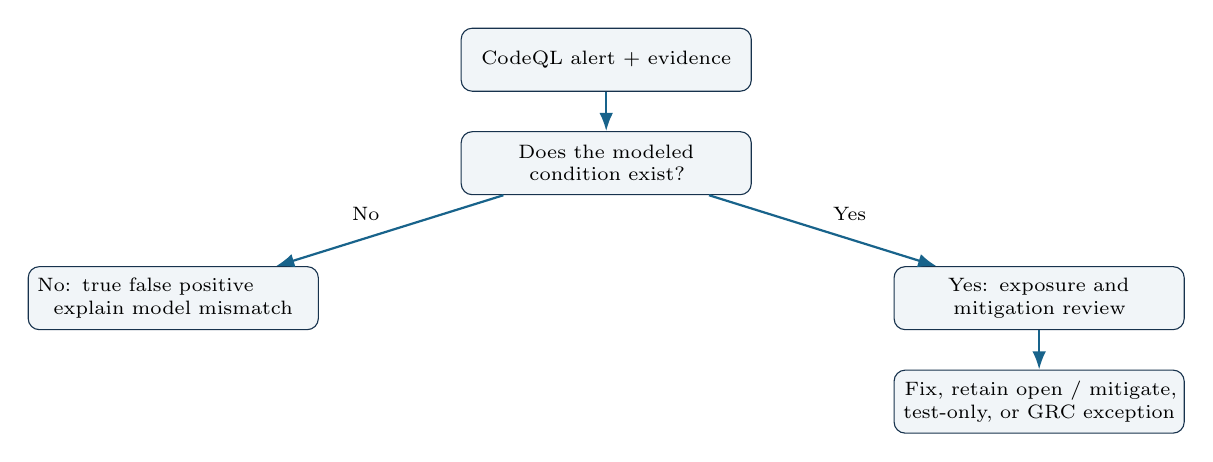
\begin{tikzpicture}[node distance=5mm and 6mm, every node/.style={font=\scriptsize}, bx/.style={draw=navy,rounded corners,fill=papergray,text width=3.45cm,minimum height=8mm,align=center}, arr/.style={-{Latex},thick,draw=azure}]
\node[bx](a){CodeQL alert + evidence};\node[bx,below=of a](b){Does the modeled condition exist?};\node[bx,below left=9mm and 18mm of b](fp){No: true false positive\newline explain model mismatch};\node[bx,below right=9mm and 18mm of b](yes){Yes: exposure and mitigation review};\node[bx,below=of yes](decision){Fix, retain open / mitigate, test-only, or GRC exception};
\draw[arr](a)--(b);\draw[arr](b)--node[above left]{No}(fp);\draw[arr](b)--node[above right]{Yes}(yes);\draw[arr](yes)--(decision);
\end{tikzpicture}\caption{Evidence-first triage decision tree}\end{figure}

\section{Disposition matrix}

\small
\setlength{\tabcolsep}{2pt}
\renewcommand{\arraystretch}{1.18}
\begin{longtable}{>{\raggedright\arraybackslash}p{0.22\linewidth}>{\raggedright\arraybackslash}p{0.38\linewidth}>{\raggedright\arraybackslash}p{0.35\linewidth}}
\toprule
\textbf{Disposition} & \textbf{Permitted when} & \textbf{Required evidence}\\
\midrule
\endfirsthead
\toprule
\textbf{Disposition} & \textbf{Permitted when} & \textbf{Required evidence}\\
\midrule
\endhead
Fix & Root cause can be corrected & Fix PR, relevant tests, scan evidence\\
Mitigated & Threat reduced by verified external control & Mitigation owner, configuration proof, test, review date\\
Used in tests & Only test-only code and no shipped reachable path & Excluded deployment and test scope evidence\\
False Positive & Source/sink path or vulnerability premise does not hold & Exact false assumption, concrete code evidence\\
Won\textquotesingle t Fix & GRC-approved, documented risk acceptance & Record ID, approval, expiry, controls, review\\
Needs investigation & Reachability/context unresolved & Assigned owner, open questions, next evidence action\\
\bottomrule
\end{longtable}
\normalsize

\section{Standardized disposition comment templates}

\begin{itemize}
\item \textbf{False positive:} ``The query assumes [X]. In [file/commit], [control/model fact] invalidates this assumption. Evidence: [test/trace]. Reviewed by [name/date].
\item \textbf{Mitigated:} ``Underlying path remains. Compensating control [ID] blocks [specific precondition]. Verified using [evidence]; owner [team]; expires/review [date].
\item \textbf{Used in tests:} ``File is confined to [test target]. Not shipped or executed in production build [proof]. Rescan when build boundaries change.
\item \textbf{GRC acceptance:} ``Exception [approval ID] covers [specific vulnerability and scope], approved [name/date], expires [date], residual risk [description].
\end{itemize}

\section{Priority and SLA}

Provide the detection score and the operational priority as separate fields. Prioritization should consider affected assets, reachability, adversary requirements, exploit maturity, environmental controls and planned remediation cost. SLAs should be policy-defined; do not assume one universal deadline for all severities. Review dismissals and mitigations when architectures or controls change.

\chapter{Remediation, Retesting, and Regression Assurance}

\section{Fix the invariant, not the alert}

\srcB\ Bishop Chapters 19--20 require justification that implementation meets design and requirements; \srcD\ Dowd Chapter 4 emphasizes reporting and remediation support. Therefore remediation evidence should close a security argument: identify the violated invariant, modify the responsible control, assert the corrected behavior, and verify every expected execution context.

\begin{figure}[htbp]\centering
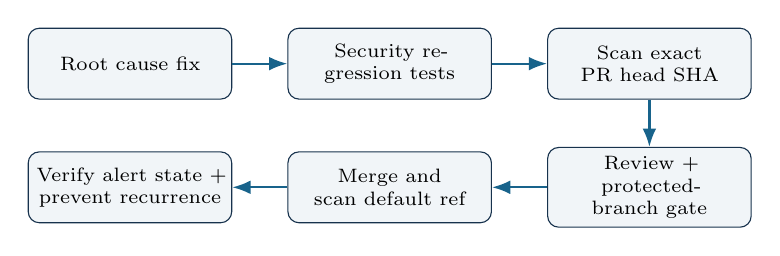
\begin{tikzpicture}[node distance=6mm and 7mm,every node/.style={font=\scriptsize},n/.style={draw=navy,rounded corners,fill=papergray,text width=2.35cm,align=center,minimum height=9mm},arr/.style={-{Latex},thick,draw=azure}]
\node[n](fix){Root cause fix};\node[n,right=of fix](test){Security regression tests};\node[n,right=of test](pr){Scan exact PR head SHA};\node[n,below=of pr](gate){Review + protected-branch gate};\node[n,left=of gate](merge){Merge and scan default ref};\node[n,left=of merge](done){Verify alert state + prevent recurrence};
\draw[arr](fix)--(test);\draw[arr](test)--(pr);\draw[arr](pr)--(gate);\draw[arr](gate)--(merge);\draw[arr](merge)--(done);
\end{tikzpicture}\caption{Pre-merge and post-merge remediation verification}\end{figure}

\section{Verification checklist}

\begin{itemize}
\item Confirm fix targets the analyzed version and relevant branch; save commit SHA.
\item Inspect changes for regression, new bypass paths and exposed failure states.
\item Run unit, integration and security regression tests, including a positive and negative case.
\item Ensure CodeQL executes on proposed fix branch/head commit prior to merge where policy requires.
\item Confirm correct query suite, all required languages and successful result upload.
\item After merge, verify default-branch analysis at merged SHA and alert state.
\item Review equivalent sinks, variants, library wrappers and sibling repositories.
\item Retain report, test output, query/pack version, reviewer, risk decision and exception IDs.
\end{itemize}

\section{When disappearance of a finding is ambiguous}

An alert can disappear because code changed, a query was removed, a file was excluded, a language extractor failed, rule metadata changed, an analysis origin disappeared, or the vulnerable path was genuinely removed. Verification must disambiguate these scenarios. A fix does not prove absence of all variants without supplementary threat analysis and tests.

\chapter{Reusable Assessment and Governance Templates}

\section{Template 1: executive assessment summary}

\small
\setlength{\tabcolsep}{2pt}
\renewcommand{\arraystretch}{1.18}
\begin{longtable}{>{\raggedright\arraybackslash}p{0.27\linewidth}>{\raggedright\arraybackslash}p{0.68\linewidth}}
\toprule
\textbf{Field} & \textbf{Fillable requirement}\\
\midrule
\endfirsthead
\toprule
\textbf{Field} & \textbf{Fillable requirement}\\
\midrule
\endhead
Application and owner & System / repository family, accountable leader\\
Period and scope & Snapshot date, assessed refs, languages, environment\\
Coverage statement & Eligible / successfully analyzed / excluded / unknown\\
Top risks & Validated critical assets, business impact, limitations\\
Disposition & Open, remediated, verified, accepted, test-only, false positives\\
Decision requested & Leadership action, owner, deadline, exception approval\\
\bottomrule
\end{longtable}
\normalsize

\section{Template 2: technical scope and boundaries}

\begin{itemize}
\item Repository URL / default branch / commit SHA / business owner / tier.
\item Components, framework versions, build modes, external integrations and dependencies.
\item Entrypoints and assets, trust boundaries, adversary assumptions and security invariants.
\item Languages queried, CodeQL version, queries/suites, configuration hash, run IDs.
\item Excluded repositories, generated code, branches and languages with justification.
\item Authorization, prohibited tests, authorized test environment and evidence retention.
\end{itemize}

\section{Template 3: coverage report}

Report each repository-language pair and require exactly one outcome: fresh successful, stale, failed, not configured, unsupported, approved excluded, or unknown. Explain the denominator and the evidence artifact for every status. Record PR-trigger coverage separately from default-branch coverage.

\section{Template 4: full vulnerability finding}

\small
\setlength{\tabcolsep}{2pt}
\renewcommand{\arraystretch}{1.18}
\begin{longtable}{>{\raggedright\arraybackslash}p{0.35\linewidth}>{\raggedright\arraybackslash}p{0.6\linewidth}}
\toprule
\textbf{Field} & \textbf{Content placeholder}\\
\midrule
\endfirsthead
\toprule
\textbf{Field} & \textbf{Content placeholder}\\
\midrule
\endhead
Finding ID / title & \rule{0pt}{13pt}\underline{\hspace{8cm}}\\
Repository / default branch / commit SHA & \rule{0pt}{13pt}\underline{\hspace{8cm}}\\
CodeQL run / query ID / query version & \rule{0pt}{13pt}\underline{\hspace{8cm}}\\
CWE / detection severity / confidence & \rule{0pt}{13pt}\underline{\hspace{8cm}}\\
Affected file / line / function & \rule{0pt}{13pt}\underline{\hspace{8cm}}\\
Entry point / attacker preconditions & \rule{0pt}{13pt}\underline{\hspace{8cm}}\\
Taint source / control / sink / relevant path & \rule{0pt}{13pt}\underline{\hspace{8cm}}\\
Security invariant and observed violation & \rule{0pt}{13pt}\underline{\hspace{8cm}}\\
Deployment context / runtime privilege & \rule{0pt}{13pt}\underline{\hspace{8cm}}\\
Observed test and reproduction scope & \rule{0pt}{13pt}\underline{\hspace{8cm}}\\
Impact, likelihood, severity rationale & \rule{0pt}{13pt}\underline{\hspace{8cm}}\\
Remediation, owner, due date & \rule{0pt}{13pt}\underline{\hspace{8cm}}\\
Disposition and GRC approval if any & \rule{0pt}{13pt}\underline{\hspace{8cm}}\\
Fix SHA / tests / CodeQL verification / review date & \rule{0pt}{13pt}\underline{\hspace{8cm}}\\
\bottomrule
\end{longtable}
\normalsize

\section{Templates 5--10: supporting records}

\small
\setlength{\tabcolsep}{2pt}
\renewcommand{\arraystretch}{1.18}
\begin{longtable}{>{\raggedright\arraybackslash}p{0.3\linewidth}>{\raggedright\arraybackslash}p{0.65\linewidth}}
\toprule
\textbf{Artifact} & \textbf{Mandatory fields}\\
\midrule
\endfirsthead
\toprule
\textbf{Artifact} & \textbf{Mandatory fields}\\
\midrule
\endhead
Data-flow evidence record & Source symbol, source trust classification, call chain, transform steps, barrier models, sink, branch conditions, diagram reference, unresolved nodes.\\
Manual validation worksheet & Candidate hypothesis, preconditions, safe fixture, expected vs observed result, command/test identifier, reviewer, timestamp, evidence hash.\\
Remediation action plan & Root cause, proposed change, accountable developer, due date, tests, dependent services, verification owner and sign-off.\\
Risk acceptance request & Scope, asset, finding identity, residual impact, compensating controls, justification, GRC approver, expiry, periodic re-review and trigger events.\\
CodeQL configuration review & Workflow SHA, triggers, languages, build mode, query suite, pack versions, permissions, extraction warnings, status check settings.\\
Assessment sign-off & Assessment lead, developer owner, independent reviewer, date, unresolved risks, approved exceptions, limitations and report reference.\\
\bottomrule
\end{longtable}
\normalsize

\chapter{Hands-On CodeQL Assessment Laboratories}

\section{Laboratory environment and safety constraints}

Exercises operate only on instructor-provided intentionally vulnerable projects, disposable containers, or isolated local repositories. Never place real keys, customer records or production endpoints in fixtures. Record your actual CodeQL CLI version before trying QL source; absence of installed tooling must be reported, not concealed.

\subsection{Lab 1: Verify CLI installation}

\textbf{Objective.} Verify CLI installation. 	extbf{Prerequisites.} CodeQL CLI installed and a scratch repo.

\textbf{Procedure.} Run 	exttt{codeql version}; record CLI and pack versions. 	extbf{Expected observation.} Tool version prints; no unexpected path shadowing.

\textbf{Acceptance criteria.} Version metadata recorded and CLI executable. \textbf{Troubleshooting.} If output differs, check installed CodeQL version, supported extractor, fixture SHA, missing imports, pack dependencies, configuration and build logs. Preserve failure evidence; do not record the exercise as successful until the relevant checks pass.

\subsection{Lab 2: Create a database}

\textbf{Objective.} Create a database. 	extbf{Prerequisites.} Small Python project with one route.

\textbf{Procedure.} Run 	exttt{codeql database create}; inspect extraction logs. 	extbf{Expected observation.} Database directory with recognized source files.

\textbf{Acceptance criteria.} Expected project functions extracted. \textbf{Troubleshooting.} If output differs, check installed CodeQL version, supported extractor, fixture SHA, missing imports, pack dependencies, configuration and build logs. Preserve failure evidence; do not record the exercise as successful until the relevant checks pass.

\subsection{Lab 3: Run standard queries}

\textbf{Objective.} Run standard queries. 	extbf{Prerequisites.} Database from Lab 2.

\textbf{Procedure.} Resolve installed Python security suite and analyze to SARIF. 	extbf{Expected observation.} Completed query evaluations and output file.

\textbf{Acceptance criteria.} Record query version, errors and result count. \textbf{Troubleshooting.} If output differs, check installed CodeQL version, supported extractor, fixture SHA, missing imports, pack dependencies, configuration and build logs. Preserve failure evidence; do not record the exercise as successful until the relevant checks pass.

\subsection{Lab 4: Read SARIF}

\textbf{Objective.} Read SARIF. 	extbf{Prerequisites.} SARIF from Lab 3.

\textbf{Procedure.} Inspect runs/tool/rules/results/locations and path traces. 	extbf{Expected observation.} Rules and locations tied to exact commit.

\textbf{Acceptance criteria.} At least one result mapped to source and version. \textbf{Troubleshooting.} If output differs, check installed CodeQL version, supported extractor, fixture SHA, missing imports, pack dependencies, configuration and build logs. Preserve failure evidence; do not record the exercise as successful until the relevant checks pass.

\subsection{Lab 5: Run candidate query}

\textbf{Objective.} Run candidate query. 	extbf{Prerequisites.} Simple 	exttt{os.open} example.

\textbf{Procedure.} Create QL file from Chapter 5; compile and evaluate. 	extbf{Expected observation.} File-open use identified independent of trust.

\textbf{Acceptance criteria.} Expected candidate shown and overbreadth explained. \textbf{Troubleshooting.} If output differs, check installed CodeQL version, supported extractor, fixture SHA, missing imports, pack dependencies, configuration and build logs. Preserve failure evidence; do not record the exercise as successful until the relevant checks pass.

\subsection{Lab 6: Write local taint query}

\textbf{Objective.} Write local taint query. 	extbf{Prerequisites.} Function parameters passed to path.

\textbf{Procedure.} Adapt query B; test direct and concatenated path. 	extbf{Expected observation.} Local taint reported when input influences sink.

\textbf{Acceptance criteria.} Positive and negative fixtures documented. \textbf{Troubleshooting.} If output differs, check installed CodeQL version, supported extractor, fixture SHA, missing imports, pack dependencies, configuration and build logs. Preserve failure evidence; do not record the exercise as successful until the relevant checks pass.

\subsection{Lab 7: Develop global path query}

\textbf{Objective.} Develop global path query. 	extbf{Prerequisites.} HTTP handler invokes file API.

\textbf{Procedure.} Adapt query C to fixture; review path nodes. 	extbf{Expected observation.} Modeled source-to-path chain visible.

\textbf{Acceptance criteria.} A sound negative fixture and limitation statement. \textbf{Troubleshooting.} If output differs, check installed CodeQL version, supported extractor, fixture SHA, missing imports, pack dependencies, configuration and build logs. Preserve failure evidence; do not record the exercise as successful until the relevant checks pass.

\subsection{Lab 8: Manual alert validation}

\textbf{Objective.} Manual alert validation. 	extbf{Prerequisites.} Intentionally unsafe Python SQL endpoint.

\textbf{Procedure.} Trace attacker input to query execution and DB permissions. 	extbf{Expected observation.} Evidence-backed exploit preconditions.

\textbf{Acceptance criteria.} Analyst determines effect without live-target exploitation. \textbf{Troubleshooting.} If output differs, check installed CodeQL version, supported extractor, fixture SHA, missing imports, pack dependencies, configuration and build logs. Preserve failure evidence; do not record the exercise as successful until the relevant checks pass.

\subsection{Lab 9: False-positive investigation}

\textbf{Objective.} False-positive investigation. 	extbf{Prerequisites.} Input sanitized by a library wrapper.

\textbf{Procedure.} Trace real sanitizer semantics and test allowed values. 	extbf{Expected observation.} Over-approximation or controlled sink established.

\textbf{Acceptance criteria.} Reason references concrete implementation and test. \textbf{Troubleshooting.} If output differs, check installed CodeQL version, supported extractor, fixture SHA, missing imports, pack dependencies, configuration and build logs. Preserve failure evidence; do not record the exercise as successful until the relevant checks pass.

\subsection{Lab 10: Repair and regression}

\textbf{Objective.} Repair and regression. 	extbf{Prerequisites.} Unsafe endpoint from Lab 8.

\textbf{Procedure.} Add bound parameters and negative tests; rerun scanner. 	extbf{Expected observation.} Regression passes and relevant alert disappears.

\textbf{Acceptance criteria.} Root cause corrected at target SHA, coverage unchanged. \textbf{Troubleshooting.} If output differs, check installed CodeQL version, supported extractor, fixture SHA, missing imports, pack dependencies, configuration and build logs. Preserve failure evidence; do not record the exercise as successful until the relevant checks pass.

\subsection{Lab 11: CodeQL + GitHub Actions}

\textbf{Objective.} CodeQL + GitHub Actions. 	extbf{Prerequisites.} Disposable training repository.

\textbf{Procedure.} Configure supported CodeQL v4 workflow and PR checks. 	extbf{Expected observation.} Successful run for PR head and default branch.

\textbf{Acceptance criteria.} Evidence for PR SHA, checks and analysis status. \textbf{Troubleshooting.} If output differs, check installed CodeQL version, supported extractor, fixture SHA, missing imports, pack dependencies, configuration and build logs. Preserve failure evidence; do not record the exercise as successful until the relevant checks pass.

\subsection{Lab 12: Organization audit dry-run}

\textbf{Objective.} Organization audit dry-run. 	extbf{Prerequisites.} Synthetic repository inventory JSON.

\textbf{Procedure.} Apply eligible/fresh/exclusion denominators and join alerts. 	extbf{Expected observation.} Counts reconcile with synthetic ground truth.

\textbf{Acceptance criteria.} No inaccessible repo mistaken for zero alerts. \textbf{Troubleshooting.} If output differs, check installed CodeQL version, supported extractor, fixture SHA, missing imports, pack dependencies, configuration and build logs. Preserve failure evidence; do not record the exercise as successful until the relevant checks pass.

\subsection{Lab 13: Final assessment report}

\textbf{Objective.} Final assessment report. 	extbf{Prerequisites.} Artifacts produced across Labs 1--12.

\textbf{Procedure.} Complete finding template, scope statement and limitations. 	extbf{Expected observation.} Reproducible evidence trail; no exaggerated claims.

\textbf{Acceptance criteria.} Independent reviewer can replay the documented checks. \textbf{Troubleshooting.} If output differs, check installed CodeQL version, supported extractor, fixture SHA, missing imports, pack dependencies, configuration and build logs. Preserve failure evidence; do not record the exercise as successful until the relevant checks pass.

\chapter{Security Principle and Vulnerability Traceability}

\section{Security theory to audit method to CodeQL evidence}

\small
\setlength{\tabcolsep}{2pt}
\renewcommand{\arraystretch}{1.18}
\begin{longtable}{>{\raggedright\arraybackslash}p{0.14\linewidth}>{\raggedright\arraybackslash}p{0.25\linewidth}>{\raggedright\arraybackslash}p{0.2\linewidth}>{\raggedright\arraybackslash}p{0.22\linewidth}>{\raggedright\arraybackslash}p{0.14\linewidth}}
\toprule
\textbf{Principle} & \textbf{Audit procedure} & \textbf{CodeQL contribution} & \textbf{Required non-query evidence} & \textbf{Textbook}\\
\midrule
\endfirsthead
\toprule
\textbf{Principle} & \textbf{Audit procedure} & \textbf{CodeQL contribution} & \textbf{Required non-query evidence} & \textbf{Textbook}\\
\midrule
\endhead
Confidentiality and information flow & Identify assets and disallowed readers; trace disclosure & Taint/data-flow query to responses/logs & Path plus authorization and classification evidence & Bishop Ch.~5,17; Dowd Ch.~2,17\\
Integrity and untrusted input & Trace attacker modifications and trust crossings & Data-flow / taint query to sensitive APIs & Input control, transformations and sink privileges & Bishop Ch.~6,17; Dowd Ch.~1,8\\
Least privilege & Review effective role and sensitive operations & Candidates for privileged APIs & IAM policy and runtime proof & Bishop 14.2.1; Dowd Ch.~9--12\\
Complete mediation & Inspect all protected object access paths & Project-specific sink inventory & Cross-role/tenant authorization tests & Bishop 14.2.4; Dowd Ch.~2,17\\
Fail-safe defaults & Force missing identity and control failures & Exception/catch/fallback candidates & Fault-injection denied-state evidence & Bishop 14.2.2; Dowd Ch.~2,7\\
Trust boundaries & Model source principal to sensitive sink & Configured source/sink taint query & Path, transport and control evidence & Bishop Ch.~1,17; Dowd Ch.~1,4\\
Memory safety & Trace allocations, writes and ownership & C/C++ API candidates & Sanitizer and boundary test results & Bishop Ch.~31; Dowd Ch.~5--7\\
Assurance & Relate requirement to implementation & Query coverage plus security invariants & Configuration, tests, independent review & Bishop Ch.~19--20; Dowd Ch.~4\\
Candidate points & Enumerate suspicious operations then backtrace & Built-in/custom query result & Verified source, path, sink and constraints & Bishop Ch.~24; Dowd 4, CP1--CP6\\
Design generalization & Reconstruct higher-level invariants & Searches only as supplements & Threat model and manual policy tests & Bishop Ch.~14; Dowd Ch.~4, DG strategies\\
\bottomrule
\end{longtable}
\normalsize

\section{Verified rule IDs versus broader catalog classes}

\small
\setlength{\tabcolsep}{2pt}
\renewcommand{\arraystretch}{1.18}
\begin{longtable}{>{\raggedright\arraybackslash}p{0.24\linewidth}>{\raggedright\arraybackslash}p{0.28\linewidth}>{\raggedright\arraybackslash}p{0.16\linewidth}>{\raggedright\arraybackslash}p{0.27\linewidth}}
\toprule
\textbf{Weakness / CWE} & \textbf{Verified rule ID} & \textbf{Language} & \textbf{Follow-up}\\
\midrule
\endfirsthead
\toprule
\textbf{Weakness / CWE} & \textbf{Verified rule ID} & \textbf{Language} & \textbf{Follow-up}\\
\midrule
\endhead
SQL injection / CWE-89 & \texttt{py/sql-injection} & Python & Trace query construction and binding\\
SQL injection / CWE-89 & \texttt{js/sql-injection} & JavaScript & Inspect ORM/raw query and parameters\\
Command injection / CWE-78 & \texttt{js/command-line-injection} & JavaScript & Confirm shell, args and reachability\\
Code injection / CWE-94 & \texttt{py/code-injection} & Python & Check eval/exec and controls\\
Code injection / CWE-94 & \texttt{js/code-injection} & JavaScript & Check interpreted context\\
Other catalog categories & No blanket ID claimed & Target-specific & Check official built-in query tables and compile custom queries\\
\bottomrule
\end{longtable}
\normalsize

\section{Boundary diagram: why a taint result is not a complete threat model}

\begin{figure}[htbp]\centering
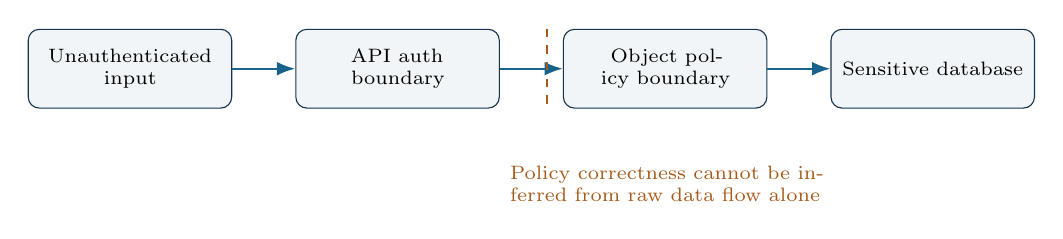
\begin{tikzpicture}[node distance=8mm, every node/.style={font=\scriptsize}, b/.style={draw=navy,rounded corners,fill=papergray,minimum height=10mm,text width=2.35cm,align=center}, ar/.style={-{Latex},thick,draw=azure}]
\node[b](guest){Unauthenticated input};\node[b,right=of guest](edge){API auth boundary};\node[b,right=of edge](policy){Object policy boundary};\node[b,right=of policy](db){Sensitive database};
\draw[ar](guest)--(edge);\draw[ar](edge)--(policy);\draw[ar](policy)--(db);
\draw[draw=warn,dashed,thick] ([xshift=-2mm]policy.west |- guest.north) -- ([xshift=-2mm]policy.west |- guest.south);
\node[below=6mm of policy,align=center,text width=4cm,font=\scriptsize\color{warn}]{Policy correctness cannot be inferred from raw data flow alone};
\end{tikzpicture}\caption{A trust-boundary crossing requires both information-flow and authorization reasoning}\end{figure}

\chapter{Reference Tables, Glossary, and Version Ledger}

\section{Terminology}

\small
\setlength{\tabcolsep}{2pt}
\renewcommand{\arraystretch}{1.18}
\begin{longtable}{>{\raggedright\arraybackslash}p{0.26\linewidth}>{\raggedright\arraybackslash}p{0.69\linewidth}}
\toprule
\textbf{Term} & \textbf{Meaning}\\
\midrule
\endfirsthead
\toprule
\textbf{Term} & \textbf{Meaning}\\
\midrule
\endhead
AST & Abstract syntax tree describing syntactic program structure\\
CFG & Control-flow graph modeling possible execution flow\\
Data flow & Modeled propagation of values through program nodes\\
Taint tracking & Modeled propagation of influence including non-value-preserving steps\\
Source / sink & Lower-trust origin and security-sensitive destination\\
Sanitizer / barrier & Operation or model that removes or blocks relevant untrusted influence\\
Path query & Query providing explanatory source-to-sink result path\\
CWE / CVE & Weakness taxonomy / public vulnerability identifier\\
SARIF & Static Analysis Results Interchange Format used for result exchange\\
SAST / DAST / IAST & Static, dynamic and interactive application security testing\\
False positive & Finding whose underlying security premise is factually incorrect\\
Complete mediation & Every security-relevant access subject to applicable enforcement\\
GRC & Governance, risk and compliance decision function\\
Assurance & Evidence-supported confidence in meeting defined security requirements\\
\bottomrule
\end{longtable}
\normalsize

\section{Acronyms}

API --- Application Programming Interface; AST --- Abstract Syntax Tree; CFG --- Control Flow Graph; CI/CD --- Continuous Integration / Continuous Delivery; CLI --- Command-Line Interface; CWE --- Common Weakness Enumeration; CVE --- Common Vulnerabilities and Exposures; GHAS --- GitHub Advanced Security (legacy/common organizational term); IAM --- Identity and Access Management; PR --- Pull Request; SAST --- Static Application Security Testing; SARIF --- Static Analysis Results Interchange Format; SQL --- Structured Query Language; TOCTOU --- Time Of Check To Time Of Use; XSS --- Cross-Site Scripting.

\section{Verification and provenance ledger}

\small
\setlength{\tabcolsep}{2pt}
\renewcommand{\arraystretch}{1.18}
\begin{longtable}{>{\raggedright\arraybackslash}p{0.36\linewidth}>{\raggedright\arraybackslash}p{0.59\linewidth}}
\toprule
\textbf{Source or tool} & \textbf{Verification status on 2026-10-16}\\
\midrule
\endfirsthead
\toprule
\textbf{Source or tool} & \textbf{Verification status on 2026-10-16}\\
\midrule
\endhead
Bishop, \emph{Computer Security}, 2nd ed. & Uploaded PDF; relevant chapters/sections cross-checked against TOC and indexed excerpts.\\
Dowd et al., \emph{Art of Software Security Assessment} & Uploaded PDF; Chapters 1--4 and catalog chapter coverage verified against table of contents and auditing excerpts.\\
CodeQL Python data-flow documentation & Live official pages reviewed; modular APIs, local taint, global ConfigSig and path query structure.\\
GitHub code-scanning docs & Live official docs reviewed: setup, compiled build modes, query sets and REST alerts.\\
CodeQL CLI / query test & Not available in execution environment; QL examples remain unexecuted.\\
GitHub Actions workflow / org audit & Example only; no repository-scoped run or authenticated GitHub request performed.\\
LaTeX and PDF & Compilation and page review reported in accompanying delivery summary.\\
\bottomrule
\end{longtable}
\normalsize

\section{Bibliography and official resources}

\begin{itemize}
\item Matt Bishop, \emph{Computer Security: Art and Science}, 2nd ed., Pearson, 2019. Chapters 1, 4--7, 14, 17, 19--20, 24--25, 31.
\item Mark Dowd, John McDonald, and Justin Schuh, \emph{The Art of Software Security Assessment: Identifying and Preventing Software Vulnerabilities}, Addison-Wesley, 2007. Chapters 1--4, 5--9, 13, 16--18.
\item GitHub, \emph{CodeQL Documentation}: \url{https://codeql.github.com/docs/}.
\item GitHub, \emph{Analyzing data flow in Python}: \url{https://codeql.github.com/docs/codeql-language-guides/analyzing-data-flow-in-python/}.
\item GitHub, \emph{Creating path queries}: \url{https://codeql.github.com/docs/writing-codeql-queries/creating-path-queries/}.
\item GitHub, \emph{GitHub CodeQL and code scanning}: \url{https://docs.github.com/en/code-security/code-scanning}.
\item GitHub, \emph{Build options for compiled languages}: \url{https://docs.github.com/en/code-security/reference/code-scanning/codeql/build-options-for-compiled-languages}.
\item GitHub, \emph{REST API endpoints for code scanning}: \url{https://docs.github.com/en/rest/code-scanning/code-scanning?apiVersion=2026-03-10}.
\item GitHub, \emph{Built-in CodeQL queries}: \url{https://docs.github.com/en/code-security/reference/code-scanning/codeql/codeql-queries/built-in-queries}.
\item GitHub, \emph{SQL query built from user-controlled sources}: \url{https://codeql.github.com/codeql-query-help/python/py-sql-injection/}.
\item GitHub, \emph{Uncontrolled command line}: \url{https://codeql.github.com/codeql-query-help/javascript/js-command-line-injection/}.
\item MITRE, \emph{CWE}: \url{https://cwe.mitre.org/}.
\end{itemize}

\section{Review exit checklist}

\begin{itemize}
\item Every finding identifies a security invariant, candidate path, and explicit degree of evidence.
\item Every coverage claim names language, branch/ref, tool/suite, execution state and denominator.
\item All exceptions have accountable owners and documented expiration/review triggers.
\item All remediation claims include tests and before/after scan context.
\item All manual-only and unmodeled risk categories remain in the assessment plan.
\item No category is claimed to have universal built-in CodeQL query coverage.
\end{itemize}

\backmatter\chapter*{Final assessment principle}\addcontentsline{toc}{chapter}{Final assessment principle}
\begin{infobox}{Evidence over dashboard counts}
A defensible application security assessment starts with a requirement, uses CodeQL to accelerate investigation, validates the actual implementation and runtime context, verifies corrective action, and declares what remains untested. Reports should be precise about uncertainty and should never substitute an alert count or a passing scan for system assurance.
\end{infobox}
\end{document}
